\documentclass[oneside, a4paper, onecolumn, 11pt]{article}

% Change this: Customize the title, author, advisor, abstract
\newcommand{\thesistitle}[0]{Improving anomaly Explanation methods on time series data}
\newcommand{\authorname}[0]{Remi Guillou}

\newcommand{\supervisor}[0]{Yanlei Diao}
\newcommand{\supervisorinstitution}[0]{École Polytechnique}

\newcommand{\abstracttext}[0]{%
The increasing amount of data being created and processed in all sectors has led to the use of automatic methods for filtering and analysing this influx of information. 
These methods often rely on complex models whose methods are intractable and as such act as "Black Boxes". Such techniques are used for monitoring traffic on many different types of servers. Anomaly detection methods are important as they make it possible to know in real time when an issue has occured. However, in order to efficiently resolve any issue, as important as detecting an anomaly is understanding why the flagged interval is anomalous.
This is where the field of Explainable AI comes into play.
In this paper, we will improve Exstream, which is a method relying on the single feature entropy measure between normal points and anomalous points to determine features that contribute the most to the anomaly and the feeature intervals where anomalies would happen.
Our contribution is twofold, first we explored the possibility of sampling normal points using the latent space from the detection method. These points would be more representative of the current anomaly and wouldn't be correlated with time. We found that the domain dependency of the data makes this technique unfeasible for our type of data.
Secondly, we showed that the scoring for different features isn't a submodular function due to correlated features but is simply increasing. We also generalized the entropy measure over multiple features which would enable the explanation of anomalies on more complex datasets where the interaction of two or more features is responsible for the anomaly.
}

\usepackage[
  left=2cm,top=2.0cm,bottom=2.0cm,right=2cm,
  headheight=17pt, % as per the warning by fancyhdr
  includehead,includefoot,
  heightrounded, % to avoid spurious underfull messages
]{geometry}


\usepackage[T1]{fontenc}
\usepackage{amstext}
\usepackage{amsmath}
\usepackage{amssymb}
\usepackage{url}
\usepackage{graphicx}
\usepackage{wrapfig}
\usepackage{enumerate}
\usepackage{paralist}
\usepackage{xspace}
\usepackage{color}
\usepackage{times}
\usepackage[colorlinks,linkcolor=blue]{hyperref}
\usepackage[colorinlistoftodos,prependcaption,textsize=normal]{todonotes}
\usepackage{pdfpages}
\usepackage{fancyhdr} %% For changing headers and footers

\usepackage{titling}
\usepackage[nottoc,numbib]{tocbibind}


\usepackage{pgfplots}
\usepackage{pgfplotstable}
\usepackage{caption}
\usepackage{subcaption}
\usepackage{tikz}
\usepackage{graphicx}

\usepackage{float}

%% \predate{}
%% \postdate{}
%% \date{}
%% \author{\authorname}


\begin{document}

%\title{\thesistitle}

%\maketitle

% Max 10 lines.
%\noindent \paragraph*{Abstract}
%\abstract

\hspace{0pt}
\vfill

\begin{center}


\includegraphics[width=0.3\textwidth]{images/logo-EP-vertical}

\vspace*{2em}
%
{\large
\textbf{\'Ecole Polytechnique}

\vspace*{1em}
\textit{BACHELOR THESIS IN COMPUTER SCIENCE}


\vspace*{3em}
{\Huge \textbf{\thesistitle}}
\vspace*{3em}



\textit{Author:}

\vspace*{1em}
\authorname{}, \'Ecole Polytechnique

\vspace*{2em}
%
{\textit{Advisor:}}

\vspace*{1em}
\supervisor{}, \supervisorinstitution{}
}

\vspace*{2em}
\textit{Academic year 2024/2025}

\end{center}

\vfill
\hspace{0pt}

\newpage

\vfill
\noindent\textbf{Abstract}\\[1em]
%
\fbox{
\parbox{\textwidth}{
\abstracttext{}
}
}
\vfill


\newpage

% Setting up the header
\pagestyle{fancy}
%\renewcommand{\headrulewidth}{0pt} % Remove line at top
%\renewcommand{\headrulewidth}{0.4pt}% Default \headrulewidth is 0.4pt
\lhead{\authorname}
%\chead{\acronym}
\rhead{\thesistitle}



\newpage
\tableofcontents
\newpage


%\pagenumbering{arabic}
\section{Introduction}
An anomaly can be defined as "an observation which deviates so much from other observations as to arouse suspicions that it was generated by a different mechanism"\cite{hawkins1980ano}. As such, Anomaly detection is the task of identifying these observations. In recent years, anomaly detection has become a core part of the machine learning landscape. It's applications are numerous and can be found in many different sectors such as healthcare \cite{medicaldeep}, finance \cite{financeanomaly} or security \cite{martins2022iot} \cite{fernandes2019network}. These method respond to the need to automate tasks that would be impossible to do manually due to the sheer amount of data on hand. In the medical domain, they can pick up on signs of a disease from medical imagery that would be impossible to detect for a human. In finance, fraudulent transaction can be pinpointed among the million happening each day. In the domain of network and server security, they enable a real time monitoring of traffic. \\
However, in each domain detecting an anomaly is only the first step. This anomalous instance must then be acted upon. In most cases a human must intervene.
It is therefore crucial to understand the reason why an anomaly was flagged. This also increases the confidence in the method and allows us to verify it's insight and provide solutions. Simple methods such as decision trees or single feature monitoring methods \cite{lstmsingle} can provide a list of features that contributed to the anomaly. 
However, with the advent of deep learning \cite{pang2021deep}, anomaly detection methods have become more complicated and less interpretable. These methods are more accurate as they can capture more complex patterns but they are also more opaque. They rely on "Black box" models that were trained to detect anomalies but give no insight into the reason why an anomaly was detected. This is where the field of anomaly explanation comes into play. The objective of anomaly explanation is to provide a human readable and actionable explanation of the anomaly. In most cases, this will be a number of features that contributed to the anomaly.\\
The objective is to provide "good" explanations. These must satisfy the following criteria: 
\begin{itemize}
  \item \textit{Conciseness:} Explanations should be short in order to be easily understood and interpreted by a human.
  \item \textit{Consistency:} The explanation must be consistent with the interpretation of it by a human. In practice, this means obtaining similar explanations for the same type of anomaly happening in the same context.
  \item \textit{Prediction power:} Explanations should be able to predict future anomalies. This is especially important in the case of time series data.
\end{itemize}
\section{Related works}
In this section we will go over previous works in the field of anomaly explanation. We can separate Anomaly explanation methods into 2 categories: model explainers and data explainers \cite{Li2023SurveyXAD} \cite{Panjei2022OutlierExplanations}.\\
\textbf{Model Explainers}\\The pipeline supports any dataset and custom preprocessing steps can be implemented. For the sake of this
paper we will be using a time series datasets consisting of traces taken from Apache Spark servers. These
traces consist of real data collected from 93 repeated executions of 10 distributed streaming applications on
a 4-node Spark cluster over a period of 2.5 months. Each of these executions includes 5 randomly selected
applications running concurrently. In total, 2,283 metrics were monitored once per second creating a dataset
totaling more than 24GB in size. For the sake of our experiments, the dataset went through some preprocessing,
cutting it down to
Model explainers are methods that provide explanations for the output of a model. These methods use the model to determine the explanation. Such methods include SHAP \cite{shap}, LIME \cite{lime} and Anchors \cite{anchors}. LIME and Anchors perturb the data around the anomaly in order to determine the closest decision boundary and therefore the features that contributed most to the anomaly. LIME uses the perturb data and outputs from the model to train a simpler more interpretable model such as a decision tree or a linear regression. Anchors on the other hand uses the predictions on the generated data to create "if then" rules called Anchors that describe the conditions under which a model consistently makes the same prediction. The predictions of LIME depend heavily on the kernel width which defines the area of interest in the generation of synthetic data making the model unstable \cite{optilime}. Anchors fixes this issue, however it becomes expensive on large datasets and is sensitive to feature selection. Overall, these two methods do not provide any theoretical guarantees as to the quality of the explanation.\\
SHAP on the other hand uses the SHAPLEY values concept from game theory to find a good set of features as explanation. This method treats the prediction task as a game, where each feature is a player that contributes to the final prediction. This method is computationally expensive and also assumes the independence of the features which isn't always the case.\\
\textbf{Data Explainers}
Data explainers do not use the model in order to provide an explanation for anomalies. These methods takes anomalous points and normal points as input and from those provide an explanation. Therefore these methods are model agnostic. Such methods include Exstream, COIN, Macrobase and lookout. Lookout is a method that attempts to find the pair of features where the anomaly is best explained is a visual manner. This is done by finding the two dimensional space where the anomalous points have the highest anomaly score as evaluated using an isolation forest. The features being returned would be the ones in which the anomaly stands out most. Macrobase uses Relative Risk Ratio, a metric from epidemiology to find the features that are most responsible for the anomaly. However, this method is limited to categorical data in its explanations. It also doesn't take into account correlation in the features being explained. Finally, in order to have good explanations, relationships between entries in the data must be known. This is not suited for raw data. COIN is a method that uses the nearest neighbors of an anomaly in order to find the best set of features to explain them. In order to do so, we find the closest cluster of normal points to our anomalous sample set. These will serve as our reference. We then fit a linear decision boundary between them. This line is constructed such that the number of non zero weights is small. These weights will indicate the features that most contribute to the anomaly. This method is reliant on a good selection of nearest cluster, this limits the local stability of the model. Moreover, the method uses a linear classifier, assuming the decision boundary is a line which isn't always the case.\\
\section{The Exathlon project}
The Exathlon project was started in 2021 as an anomaly detection and explanation benchmark \cite{Exathlon}. The github repository implements a pipeline that implements all needed steps from preprocessing of the data to training and evaluating methods for detecting and explaining anomalies. The full pipeline can be seen in \autoref{fig:pipeline}.
\subsection{Dataset}
The pipeline supports any dataset and custom preprocessing steps can be implemented. For the sake of this paper we will be using a time series datasets consisting of traces taken from Apache Spark servers. These traces consist of real data collected from 93 repeated executions of 10 distributed streaming applications on a 4-node Spark cluster over a period of 2.5 months. Each of these executions includes 5 randomly selected applications running concurrently. In total, 2,283 metrics were monitored once per second creating a dataset totaling more than 24GB in size. For the sake of our experiments, the dataset went through some preprocessing, cutting it down to 237 features. It can be noted that this preprocessing step is done automatically in the pipeline.
The dataset consists of 59 undisturbed traces and 34 disturbed traces constituting 97 anomaly intervals. There are 6 types of anomalies that were artificially produced. These are the following: 
\begin{itemize}
    \item T1: bursty input : temporarily increase the input rate by a given factor for a duration of 15-30 minutes.
    \item T2: bursty input until crash : Similar to T1 except the input rate is maintained at a high rate until experiencing a crash due to lack of memory.
    \item T3: stalled input : artificially set the input rates to 0 for about 15 minutes.
    \item T4: CPU contention : consume all CPU cores on a given Spark
    node.
    \item T5: driver failure : artificially failing the driver processes.
    \item T6: executor failure : artificially failing the executor processes.
    \item T7 : a mix of unknown types of anomalies.
\end{itemize}
The data is processed and then turned into a \textit{window dataset} which transforms the data into a sliding window format in order to detect the anomalies.
\subsection{Anomaly detection}
The anomaly detection consists of three steps. First training the \textit{window model}. This model gives an anomaly score to a window of a certain size. Then following the "Unifying anomaly detection method" introduced by Vincent Jacob \cite{Divad}, we obtain an "Online" anomaly scoring function which given the scoring for windows, attributes a score for each point. This scoring function is used to determine a threshold above which points will be labelled as anomalies in the anomaly detection step.\\
Many different models belonging to various families of methods \cite{Schmidl2022} are implemented and ready to be evaluated.\\
Such methods include among others: pca, xgboost, Autoencoder, Variational Autoencoder, LSTM, deep SVDD, deep SAD, iForest...\\
The most recent and best model on this dataset is Divad.
\subsubsection{Divad}
\label{subsec:divad_domain}
\begin{figure}[h]
  \centering
  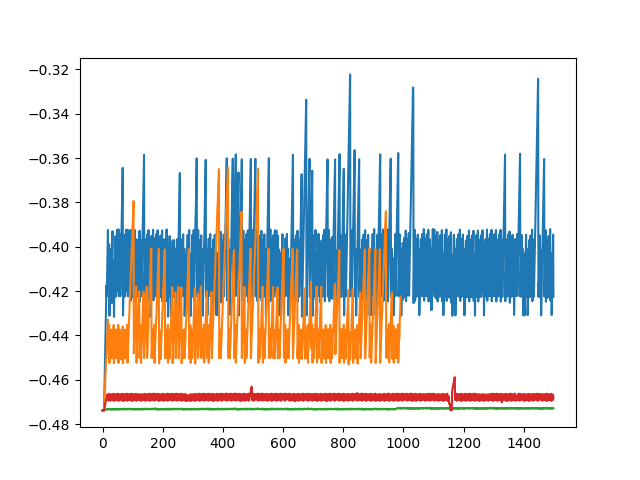
\includegraphics[width=0.5\textwidth]{images/domains.png}
  \caption{Plot of feature "driver\_BlockManager\_memory\_memUsed\_MB\_value" for 4 normal traces over time.}
  \label{fig:domains}
\end{figure}
Divad is an anomaly detection method based around a VAE architecture \cite{Divad}. This method was created to address the difference in the behaviour of traces based on the parameters and properties of the Spark application they were run on. We will call "Domain" the context in which the application is run. This context is characterised by the following elements: processing period, number of active executors, memory profile and input rate.\\\\
The different domains pose a real problem when trying to identify anomalies. A certain behavior can be considered anomalous in one domain but not in another.
The limited amount of data also makes it impossible to train a model for each domain. Therefore we need a method that can detect anomalies and generalize to new domains. This is Divad.\\\\
The way it works is by assuming two independent priors that define the data z. The first prior is the class y, either anomaly or normal. The second prior is one that encodes the domain of the point \autoref{fig:divad_assum}. Therefore we are assuming that the points can be generated from their class and their domain and that these two priors are independent.\\
The objective is thus to approximate these prior spaces from the data. In order to do so, Divad employs a Variational Autoencoder structure with two independent encoders and one decoder. The first encoder is meant to capture the Class information and the second the Domain information \autoref{fig:divad_simple} \autoref{fig:divad_arch}. This is done using well chosen error functions.\\
We therefore end up with two latent spaces: $z_y$ and $z_d$ that contain respectively information about the class and the domain of the data. We then use these two latent space to reconstruct the data.
\begin{figure}[H]
  \centering
  \begin{subfigure}{0.6\textwidth}
      \centering
      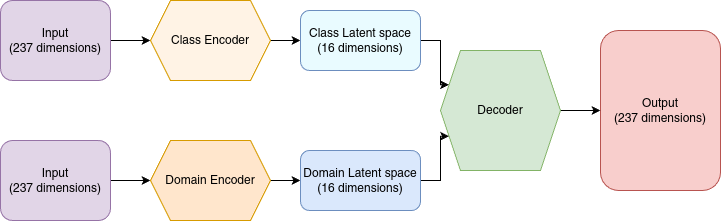
\includegraphics[width=\linewidth]{images/divad_simple.png}
      \caption{Simplified representation of Divad}
      \label{fig:divad_simple}
  \end{subfigure}
  \begin{subfigure}{0.2\textwidth}
      \centering
      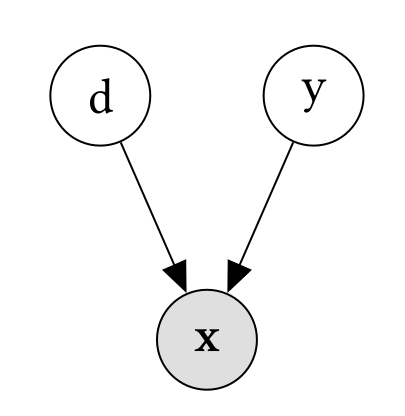
\includegraphics[width=\linewidth]{images/divad_assum.png}
      \caption{ x depends on its domain d and class y.}
      \label{fig:divad_assum}
  \end{subfigure}
  \caption{Divad architecture}
\end{figure}
We get an anomaly score by comparing the class latent space with what we would expect from the normal class. This is done by computing the KL divergence between the two distributions.\\
\subsection{Anomaly Explanation}
The anomaly explanation step will be the main focus of this paper. The objective of this step is to give a human readable and actionable explanation of the anomaly. This can be done in many ways such as lists of feature importance or plots as we have seen in the related works. In this paper, the focus will be on the Exstream method. For each anomaly, this method will output the features that cause the anomaly as well as the intervals where the anomaly is happening.\\
The explanation is given as a boolean expression in Conjunctive Normal Form. It consists of a conjunction of clauses, where each clause is a disjunction of predicates. Each predicate follows the form \{v o c\}, where v represents a feature, c is a constant, and o is one of the five operators: $o\in\{>, <, \geq, \leq, =\}$.\\
For example an explanation for an anomaly could be the following: (feature1 > 0.5) $\lor$ (feature1 < 0.8) $\land$ (feature2 = 0.7).\\
In practice, the explanation is given as a json file with one entry per anomalous interval in the following format:
\begin{verbatim}
  {
    "Trace":{
      "Anomaly number and type":{
          "feature_to_importance":{
              "feature 1": score 1
              "feature 2": score 2,
          },
          "feature_to_intervals":{
              "feature 1":[
                  [
                      start,
                      end,
                      include start,
                      include end
                  ]
              ],
              "feature 2":[
                  [
                      start,
                      end,
                      include start,
                      include end
                  ],
                  [
                      start,
                      end,
                      include start,
                      include end
                  ]
              ]
          }
      },
      ...
    }
    ...
  }
\end{verbatim}
\label{explanation_format}
There previously existed two versions of Exstream. The original version was introduced by Haopeng Zhang, Yanlei Diao and Alexandra Meliou  in 2017 \cite{Exstream}. It was then worked uppon by Mija Pilkaite during her Bachelor thesis \cite{MijaExstream} and finally refined and improved by Clement Martineau \cite{ClementExstream}.\\
\subsubsection{Original Exstream}
\begin{figure}[h]
  \centering
  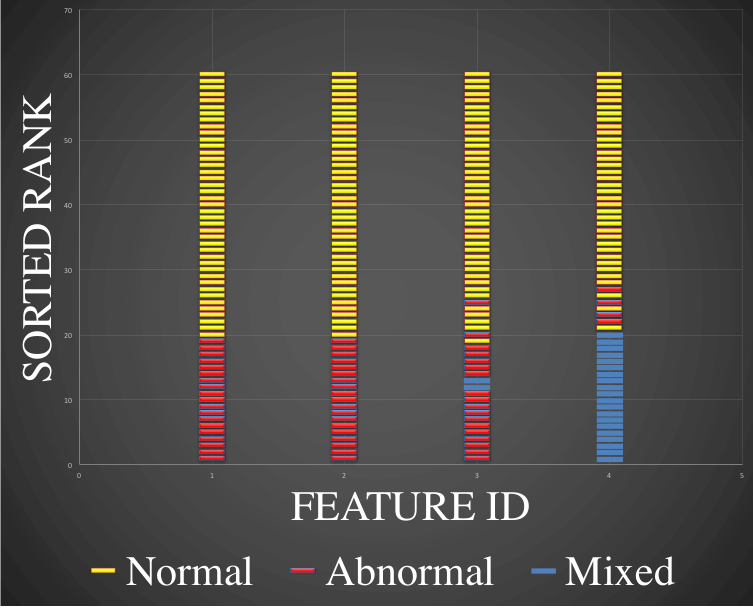
\includegraphics[width=0.5\textwidth]{images/exstreamplot.png}
  \caption{Visualization of the segments of 4 features. The red points are the anomalous points,the yellow points are the normal points and the blue are mixed. Segments are continuous points of the same colour.}
  \label{fig:exstreamplot}
\end{figure}
Originally, Exstream was created to provide a rigorous and formal method for providing short and human readable explanations for anomalies. This method presents the challenge of finding the optimal explanation to an anomaly as a submodular optimization problem. The intuition behind this model is that adding features to our explanation has a diminishing return. This is because the more features we add, the less information new features will provide.\\
Submodular optimization being NP-hard, a heuristice was therefore introduced to solve the problem. This method relies on Entropy to compute single feature scores.\\\\
We start with two sets of points $S_a$ and $S_n$ containing respectively the anomalous and normal points.
For each feature $f_i$, we will sort the points in $S_a$ and $S_n$ and merge them into one set. We will then define segments on this set as neighbouring points of the same class.

We will compute a segmentation entropy defined as follows:
If there are n segmentations, and $p_i$ represents the ratio of data points included in the ith segmentation, the segmentation entropy is:
\begin{equation}
    H_{segmentation} = \sum_{i=1}^{n} p_i \log(\frac{1}{p_i})
\end{equation}

Exstream was originally aimed at categorical data. Therefore there can be features with values that belong both to anomaly and to normal points. We need to penalize these features. This is done by giving the worst score to those points of mixed class. Let $c_i$ be a mixed interval and $c_i^*$ be the segment rearanged in its worst ordering.\\
Then the maximum entropy is defined as:
\begin{equation}
    H_{max} = \sum_{i=1}^{n} H_{segmentation}(c_i^*)
\end{equation}
Finally, we normalize the score by the class entropy to get a value between 0 and 1. The class entropy is defined as follows:
Let $|S_a|$ and $|S_n|$ be the number of points in $S_a$ and $S_n$ respectively. $p_a = \frac{|S_a|}{|S_a| + |S_n|}$ and $p_n = \frac{|S_n|}{|S_a| + |S_n|}$. The class entropy is then:
\begin{equation}
    H_{class} = p_a \log(\frac{1}{p_a}) + p_n \log(\frac{1}{p_n})
\end{equation}

The final score for a feature is then:
\begin{equation}
    score(f_i) = \frac{H_{segmentation} + H_{max}}{H_{class}}
\end{equation}
This score reflects the segmentation of the feature with respect to anomaly and normal classes. The higher the score, the more separated normal and anomaly classes are. For example a feature with a score of 1 would have all the anomaly points in one segment and all the normal points in another. As we can see in \autoref{fig:exstreamplot}, the first two features have a score of 1. The third a score of 0.31 and the fourth 0.18.\\
Exstream selects the best features based on reward leap filtering. It also provides methods to filter out redundant features using correlation clusters. It also removes "false positive" features which are defined as those with excessively large standard deviation or that tend to only increase or decrease on both the normal and anomalous interval.\\
\subsubsection{Exstream using Bins}
\begin{figure}[H]
  \centering
  \begin{subfigure}{0.3\textwidth}
      \centering
      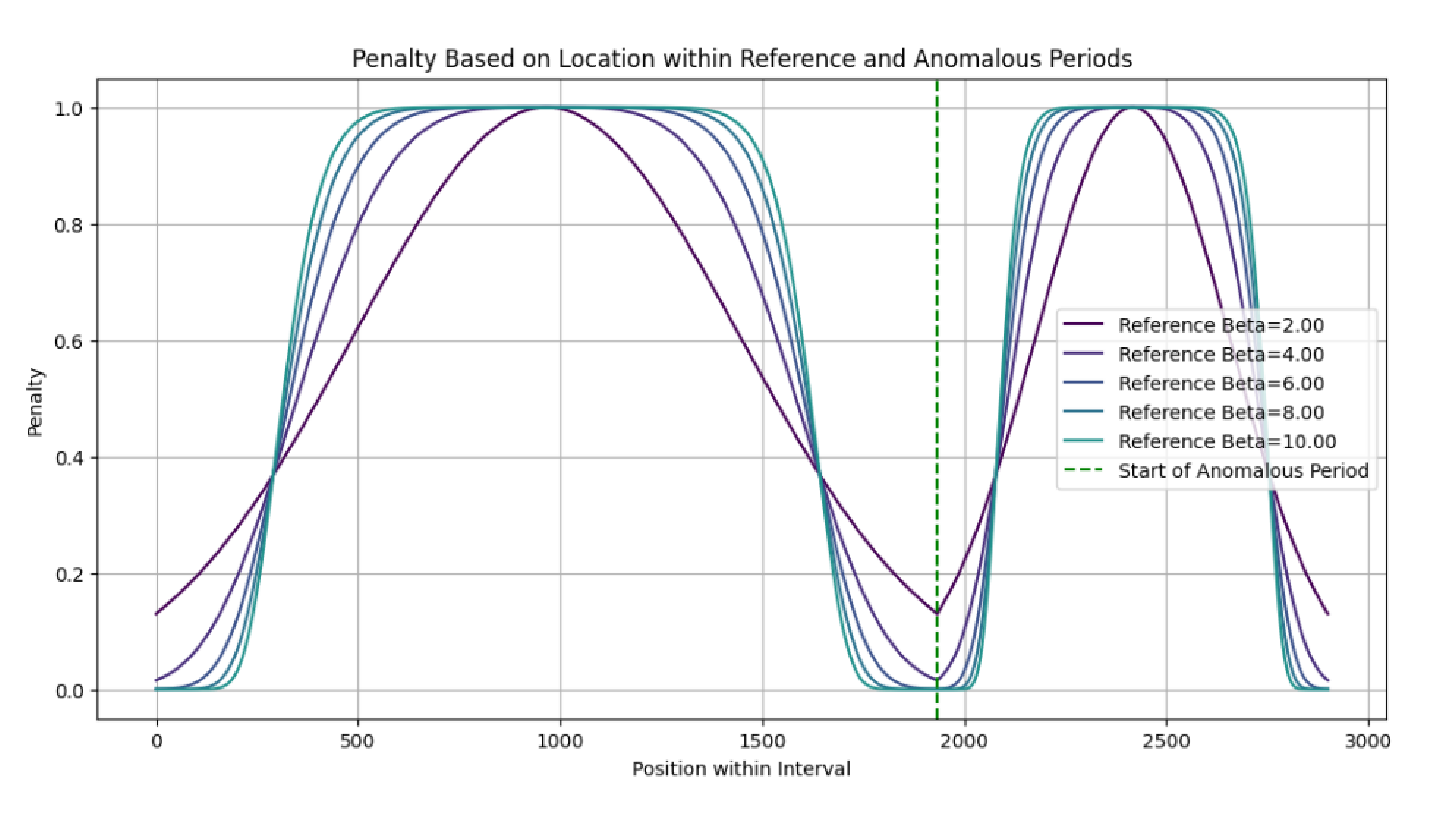
\includegraphics[width=\linewidth]{images/bin_1.png}
      \caption{Changes based on beta values}
  \end{subfigure}
  \begin{subfigure}{0.3\textwidth}
      \centering
      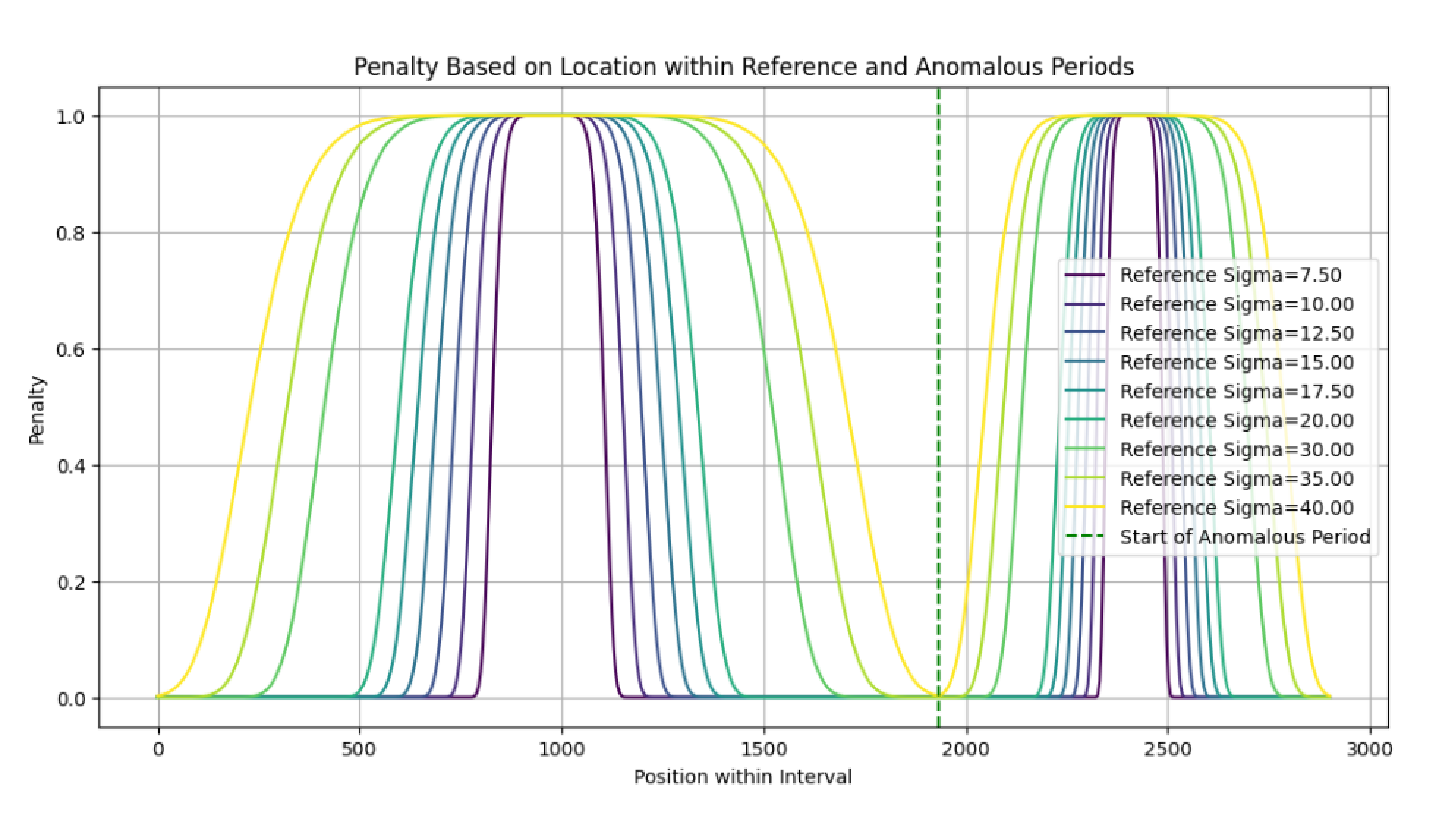
\includegraphics[width=\linewidth]{images/bin_2.png}
      \caption{Changes based on sigma}
  \end{subfigure}
  \caption{Normal distributions used to weigh points.}
\end{figure}
An attempt to improve Exstream was made by Mija Pilkaite during her Bachelor thesis \cite{MijaExstream}. The first idea was to use bins to discretize the data. This would make the method more suitable for continuous data. The values of each feature would be divided into b bins. Each bin would be marked as either Normal, Anomalous or Mixed. The entropy would then be computed on these bins instead of points. 
The second idea was to reduce uncertainty in the anomalous interval boundaries. Even when using ground truth segments with anomalous intervals marked by hand, there is always some uncertainty as to exact endpoints of the intervals. \\
In order to minimize this labeling uncertainty, the points would have different weights in the computation of the entropy depending on their position in the trace. This weighting would be done using a Gaussian distribution centered around the middle of the interval as such:
% Equation
\[
w_t =
\begin{cases}
\exp \left( - \left( \frac{| position - \frac{interval\_length}{2} |}{\sigma \times \frac{interval\_length}{100}} \right)^{\beta} \right), & \text{if } 0 \leq position \leq interval\_length \\
0, & \text{otherwise}
\end{cases}
\]
This was further developed by Clement Martineau who corrected some issues and improved the method in higher dimensions.\\
\subsubsection{Metrics}
The Exathlon pipeline provides a set of metrics to evaluate the performance of the explanation models. These metrics are the following:
\begin{enumerate}
  \item ED1: These metrics are based on local behavior of the anomaly explanation.
  \begin{itemize}
    \item Time: The time taken to compute the explanation.
    \item Size: The size of the explanation. This is the number of features contained in the explanation.
    \item Perturbed Size: Size of the explanation after perturbation. A perturbation is defined as a random sampling of 80\% of the data in the normal and anomalous intervals. The perturbed size is the number of features in the explanation of a trace having been perturbed.
    \item Instability: A measure of the difference in the explanation before and after a perturbation. A high instability means that the explanation is not locally stable.
    \item F1 Score, Precision, Recall: These metrics are computed by giving an explanation on a randomly sampled 80\% of the normal and anomalous data and then testing the explanation on the remaining 20\%. The testing is done on the intervals being returned as being anomalous. From them a Precision and Recall score are computed. The F1 Score is the harmonic mean of the two. Similarly as for the instability, the random sampling and evaluation are carried out 5 times and the average is taken.
  \end{itemize}
  \item ED2: These metrics are based on global behavior of the anomaly explanation.
  \begin{itemize}
    \item Discordance: This is the degree of disagreement between the explanation for anomalies of the same type. This measure is computed for each type of anomaly as the entropy of the number of each feature found in all explanations of this type. The discordance is then normalized by the average number of features in an explanation.
    \item F1 Score, Precision, Recall: these metrics are computed by getting an explanation on one sample and evaluating it on all the other test samples of the same trace. Similarly as for ED1, these scored are computed on the intervals being returned as being anomalous. The F1 Score is the average of the F1 Scores computed on each other test sample.
  \end{itemize}
\end{enumerate}
These metrics are all computed for each type of anomaly as well as for the whole dataset.\\
It is important to note the limitations of these metrics. For anomaly explanation contrary to anomaly detection, there is no ground truth. Therefore getting perfect Discordance and Stability does not imply that the explanation is good. For example a method returning \textit{feature1} as an explanation every time would get perfect scores for both metrics. This is especially important for explanation methods that do not provide intervals but only important features. This is why inspecting specific examples and determining if the explanation provided is relevant is important.\\\\
Overall, these metrics are very useful in comparing different methods. However, they should be taken with a grain of salt and the results should be interpreted with caution\\  
\subsubsection{Evaluating current methods}
\begin{table}[h]
  \centering
  \begin{tabular}{|c|c|c|c|c|c|c|}
      \hline
      Methods & Time & Length & Instability & Discordance & ED1 F1 Score & ED2 F1 Score\\ 
      \hline
      Exstream  & 1.5  & 1.6  & 2.26  & 7.71 & 0.88 & 0.87  \\ 
      Exstream 95\%  & 1.35  & 2.1  & 2.08  & 6.59 & 0.87 & 0.93\\ 
      Exstream 90\%  & 1.2  & 2.4  & 1.88  & 6.04 & 0.88 & 0.92\\ 
      Exstream 80\% & 1.1 & 3.4 & 2.0 & 5.5 & 0.88 & 0.90 \\
      Exstream Bins  & 140.7  & 4.3  & 1.5  & 6.16 & 0.79 & 0.72 \\ 
      \hline
  \end{tabular}
  \caption{Evaluation of Exstream methods}
  \label{tab:example}
\end{table}
We start by evaluating the current existing Exstream methods and find little improvement in the Exstream Bins method over the orinal. The instability and discordance are reduced but so is the F1 Score in both ED1 and ED2 settings. The length of the explanation is also increased. The true bottle neck however is the runtime which is multiplied by a factor of 100. This limits its use in real time monitoring. The delay is due in part to poorly optimized code but also to the apparent complexity of the algorithm in processing the bins. The algorithm was also never evaluated on the entirety of the Exathlon data and only on a subset with shorted traces which limited the impact on performance.\\ 
In order to compare, we also evaluate the original Exstream while removing the first and last 5\% and 2.5\%normal and anomalous points. This in practice removes the uncertainty linked to the labeling at the boundaries of the intervals while keeping the algorithm simple and preserving speed. This new method improves the instability and discordance over Exstream while keeping a high F1 Score. The length of the explanation increases. This can be explained by the fact that labeling noise initially created segmentation in well separated features. Removing the noise leads to more well separated features to explain the data.  It can also be noticed by looking at the examples that the explanations are more confident and more relevant. There are many more features that are selected with a confidence score of 1. \\
For example, trace 5\_5\_1500000\_5\_3\_9\_91 anomaly 1\_T6 as seen below. Using all points, the responsible feature is 
"driver\_LiveListenerBus\_listenerProcessingTime\_org\_apache\_spark\_scheduler\_EventLoggingListener\\\_stddev" with a score of 0.054. Meanwhile using 95\% of the data it is a slightly longer explanation with features : "avg\_NettyBlockTransfer\_shuffle-server\_usedDirectMemory\_value" and "avg\_jvm\_direct\_capacity\_value" with both a score of 1.\\

\begin{figure}[H]
  \centering
  \begin{subfigure}{0.3\textwidth}
      \centering
      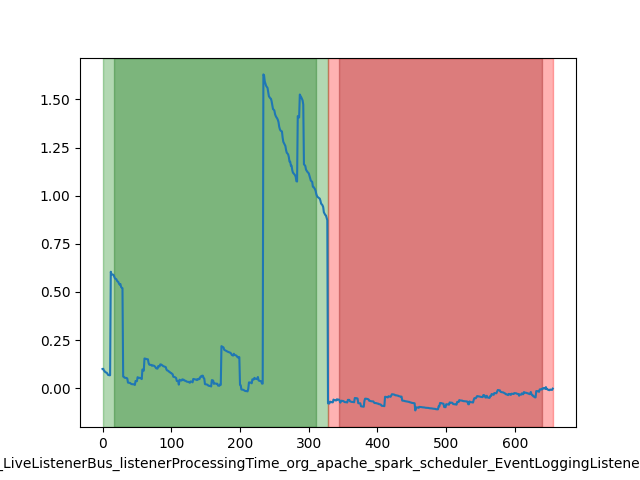
\includegraphics[width=\linewidth]{images/ex_remove5bad.png}
      \caption{Exstream responsible feature}
  \end{subfigure}
  \hfill
  \begin{subfigure}{0.3\textwidth}
      \centering
      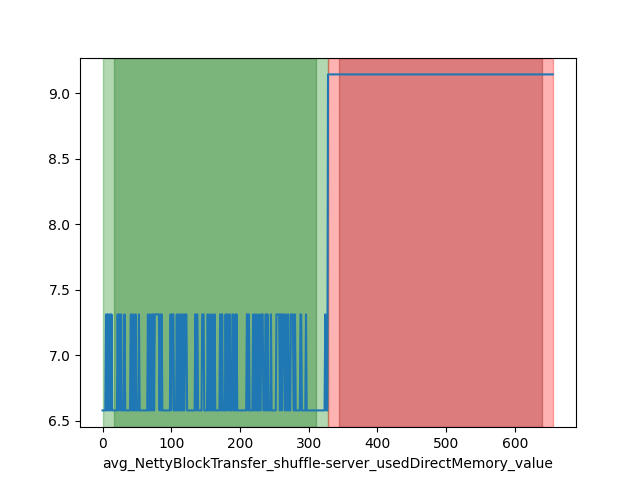
\includegraphics[width=\linewidth]{images/ex_remove5.png}
      \caption{Exstream 95\% responsible feature 1}
  \end{subfigure}
  \hfill
  \begin{subfigure}{0.3\textwidth}
      \centering
      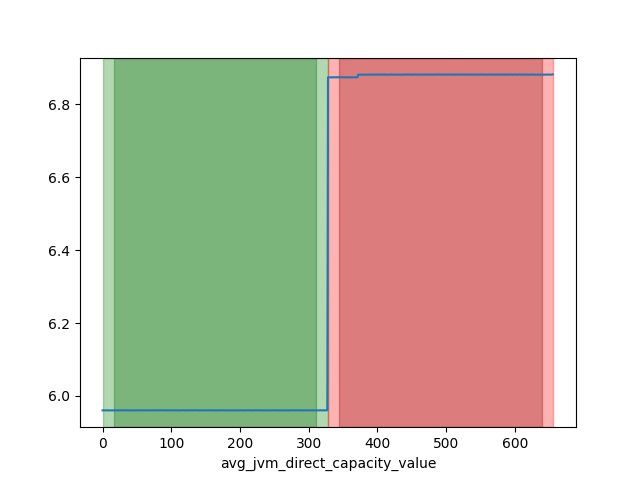
\includegraphics[width=\linewidth]{images/ex_remove52.png}
      \caption{Exstream 95\% responsible feature 2}
  \end{subfigure}
  \caption{Responsible features for anomaly at Trace 5\_5\_1500000\_5\_3\_9\_91 anomaly 1\_T6. Green are normal points, red are anomalous points. Lighter parts are the 5\% removed.}
\end{figure}
Another element that shows the improvement when discarding 5\% of the data is the length of the explanation file. When evaluating the length of the explanation, the metric is the number of relevant features being selected. This discards completely the number of intervals for each feature. The explanation file contains both features and intervals as seen previously \autoref{explanation_format}. The length of the explanation file is therefore a good metric when evaluating the method on the same anomalies. In the case using all points, this file has 22434 lines. When using 95\% of the data it has 3720. This reflects the poor separation observed in many traces which require many intervals to describe their behavior. Using bins, the explanation file has 14380 lines.\\


\section{Objectives}
The focus of this paper will be to improve Exstream. The version we intend to work on will be the original version. This choice is motivated by a few reasons. \\
First, looking at the metrics and inspecting a few examples shows that the version using bins does not offer any significant improvements. 
Secondly, the time to run is multiplied close to 100 times. This performance issue is partly caused by unoptimized code and partly by an overcomplicated algorithm. The algorithm was also never previously evaluated as part of the Exathlon pipeline and only on a subset of the available data. 
The complexity of the algorithm makes it very rigid and hard to modify in relevant ways while at the same time the runtime is too long to be used in a real time setting.\\\\
There are two ways in which we can improve Exstream. The first is to improve the sample set. The second is to improve the algorithm being used. In this paper we will address both of these points with varying degrees of success.\\
\section{Improving the sample set}
A problem noticed when evaluating Exstream on the Exathlon data is that the normal points used are not necessarily the most representative of the current anomaly. This is due to the fact that the normal points selected are right before the anomaly. There is therefore a strong correlation between these points and time. The most obvious examples of this are features that are only increasing or decreasing over the normal and anomalous intervals. The segmentation of these features will be perfect and the score will be 1 while these features aren't relevant explanations for the anomaly.\\
This specific case of time correlation is already addressed in the original Exstream paper using false positive filtering. However less obvious cases of correlation are not addressed and can lead to wrong explanations.\\
At the same time we will attempt to get sample of normal points "closer" to the anomaly. This sample should be more representative of the current anomaly and only the relevant features that induced the anomaly will significantly change. This should enable a better explanation.\\
\subsection{Sampling using the latent space}
\begin{figure}
  \centering
  \begin{subfigure}{0.3\textwidth}
      \centering
      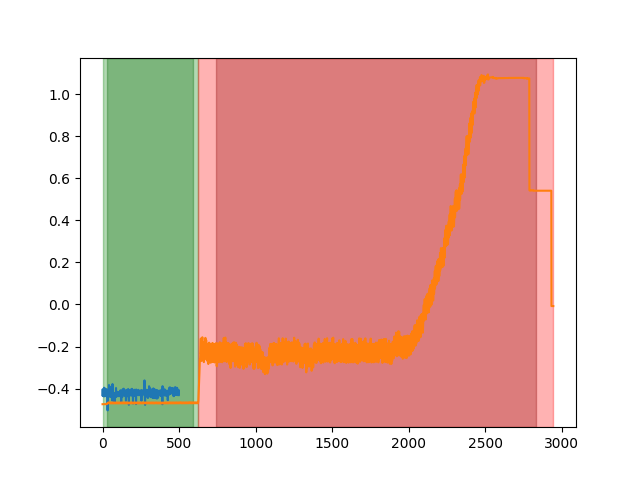
\includegraphics[width=\linewidth]{images/reconstruction/dim_1.png}
      \caption{Feature 1}
  \end{subfigure}
  \hfill
  \begin{subfigure}{0.3\textwidth}
      \centering
      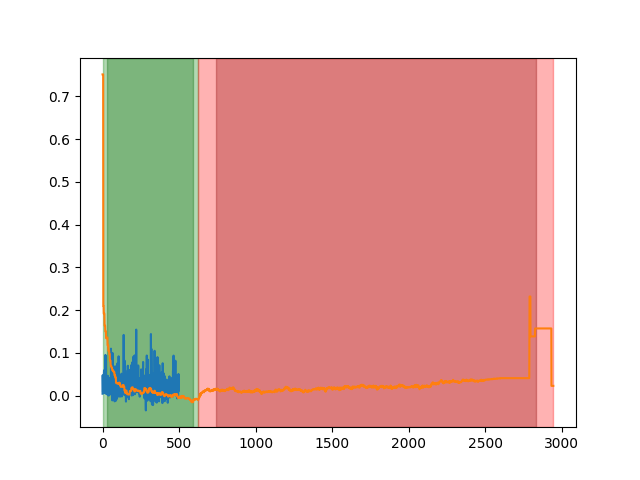
\includegraphics[width=\linewidth]{images/reconstruction/dim_14.png}
      \caption{Feature 14}
  \end{subfigure}
  \hfill
  \begin{subfigure}{0.3\textwidth}
      \centering
      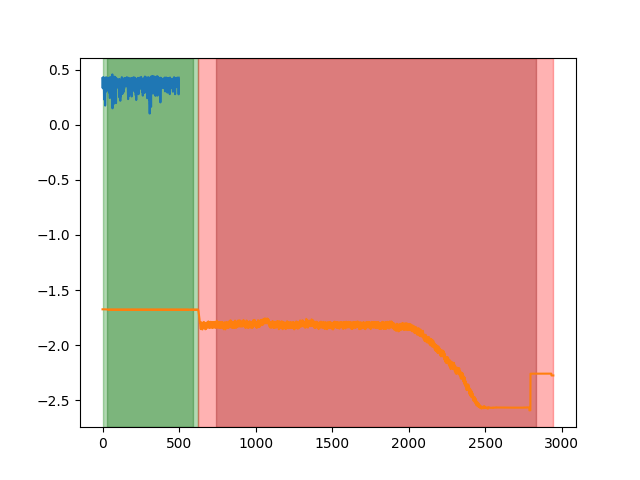
\includegraphics[width=\linewidth]{images/reconstruction/dim_3.png}
      \caption{Feature 3}
  \end{subfigure}
  \begin{subfigure}{0.3\textwidth}
    \centering
    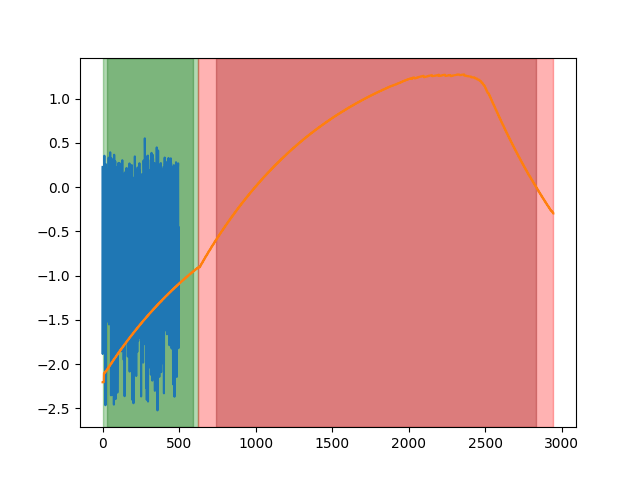
\includegraphics[width=\linewidth]{images/reconstruction/dim_6.png}
    \caption{Feature 6}
\end{subfigure}
\begin{subfigure}{0.3\textwidth}
  \centering
  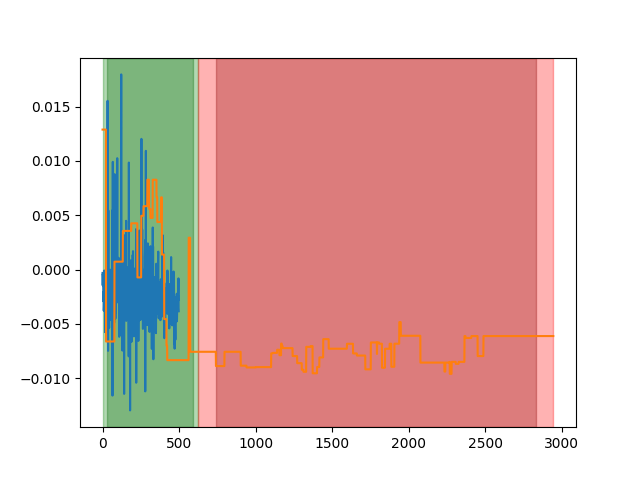
\includegraphics[width=\linewidth]{images/reconstruction/dim_12.png}
  \caption{Feature 12}
\end{subfigure}
\begin{subfigure}{0.3\textwidth}
  \centering
  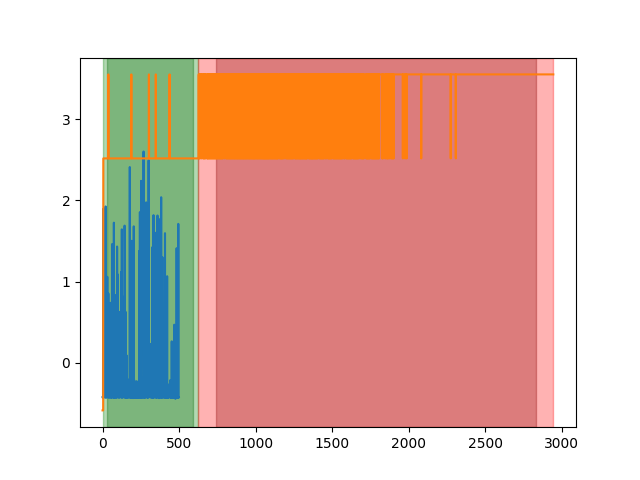
\includegraphics[width=\linewidth]{images/reconstruction/dim_20.png}
  \caption{Feature 20}
\end{subfigure}
  \caption{Plot of three features. Green is the normal interval and red the anomalous one. The blue points are reconstructed samples that are "close" to the anomaly, as detailed below.}
  \label{fig:reconstruction}
\end{figure}
The latent space of a VAE has a well defined structure. The normal points will be distributed following a normal distribution. The space is created such that relevant features to the detection of the anomaly are captures. Therefore the hope is that normal points close to anomalous points are similar to those. Moreover, the difference between those points will be marked more strongly by the features that caused the anomaly. Features unrelated to the anomaly will have similar values while those implicated will be different. This also enables a search on all points for a reference set and not only on preceding points.\\
The problem with this method is the existence of different domains in our data. As stated above \autoref{subsec:divad_domain}, a datapoint might be normal in a specific domain while considered anomalous in another. Therefore the points closest to the anomaly in the latent space might belong to a different domain and therefore not be well suited to interpret the anomaly. In order to address this issue, we will make use of the model to reconstruct the data in the right domain. \\
As stated above, Divad uses two encoders, one to extract a latent space encoding the class and the other the domain. These two latent spaces are combined in the decoder to reconstruct the data. We can therefore extract the domain latent space of the anomaly and use it to reconstruct points in the right domain. These points will then be used as the normal points in the explanation.\\
In practice, some features are well reconstructed, while others not so well. This is due to the fact that the model is not perfect and that some features are more relevant to the anomaly than others. This can be seen in \autoref{fig:reconstruction}. This is especially true in categorical data such as feature 20.\\
The results of this method are as follows:
\begin{table}[h]
  \centering
  \begin{tabular}{|c|c|c|c|c|c|c|}
      \hline
      Methods & Time & Length & Instability & Discordance & ED1 F1 Score & ED2 F1 Score\\ 
      \hline
      Exstream  & 1.5  & 1.6  & 2.26  & 7.71 & 0.88 & 0.87  \\ 
      Exstream 95\%  & 1.35  & 2.1  & 2.08  & 6.59 & 0.87 & 0.93\\ 
      Exstream 90\%  & 1.2  & 2.4  & 1.88  & 6.04 & 0.88 & 0.92\\ 
      Exstream 80\% & 1.1 & 3.4 & 2.0 & 5.5 & 0.88 & 0.90 \\
      Exstream Reconstruction 100\% & 5.2  & 1.6  & 2.77  & 8.56 & 0.79 & 0.81  \\
      Exstream Reconstruction 95\%  & 4.3  & 1.8  & 3.17 & 7.08 & 0.78 & 0.87\\ 
      Exstream Reconstruction 90\%  & 4.3  & 2.2  & 2.87  & 5.59 & 0.79 & 0.86\\ 
      Exstream Reconstruction 80\% & 4.2 & 2.6 & 2.04 & 5.65 & 0.79 & 0.84 \\ 
      \hline
  \end{tabular}
  \caption{Evaluation of the Exstream method using reconstructed points}
  \label{tab:example}
\end{table}
The results are not as good as expected. The instability and discordance are increased while the F1 Score is decreased. The length of the explanation is however similar. Using reconstructed points also raises another issue which is our confidence in the explanation. If the points being reconstructed are far from the truth, the method might miss some features that would otherwise be good explanation. It is impossible to have a sense of the quality of the explanation.\\


\section{Generalizing Exstream to Higher dimensions}
As seen earlier, exstream computes entropy on a single feature. This is a limitation as anomalies can be caused by the interaction of two or more features. This method was initially given as a way of finding an approximation to the problem of finding the best set of features to explain an anomaly. This problem was believed to be submodular.\\
In this section we will start by showing that this problem isn't submodular. We will then present multiple ways the entropy measure can be generalized to multiple dimensions. We will then evaluate these methods and empirically show benefits that are derived from using them.\\
\subsection{Submodular optimization}
Let $A$ be a set and $\mathbb{A} = \mathcal{P}(A)$ be its powerset. The set function $f: \mathbb{A} \rightarrow \mathbb{R}$ is submodular if $\forall X, Y \subseteq \mathbb{A}$, 
\begin{align*}
    f(X) + f(Y) \geq f(X \cup Y) + f(X \cap Y)
\end{align*}
It is also equivalent to saying $\forall X \subseteq Y \subseteq \mathbb{A}, \forall x \in \mathbb{A} \setminus Y$: 
\begin{align*}
    f(X \cup \{x\}) - f(X) \geq f(Y \cup \{x\}) - f(Y)
\end{align*}
The submodularity of a function reflects the diminishing return of adding elements to a set. This property is very useful in optimization problems as it allows for the use of greedy algorithms to obtain an approximate of the solution \cite{niazadehsubmodular}.\\
This property has been shown to occur in feature selection problems but only in the case where features are independent \cite{submodular_independent}. This is not the case for our data.\\
Let us show visually that the submodularity property does not hold. We start by formally defining our setting:\\
We denote the features by numbers from 1 to 237. Let $D=[1, 237]$ be the set of all features. Then $\mathbb{D} = \mathcal{P} (D)$ be the powerset of $D$. We further annotate each interval of Anomalous and Normal points $(N_i, A_i)$ by a number $i$. We then define the function $f_i: \mathbb{D} \rightarrow [0, 1]$ as a function computing the entropy of the segmentation of the features being passed for the pair $(N_i, A_i)$.\\
We need the function $f_i$ to be submodular for each pair $(N_i, A_i)$. Therefore let us present an example for which this property does not hold, see \autoref{fig:exstream2dplot}. Here in either dimension there will be very high segmentation. However, considering both features we see a clear separation between the anomalous and normal points. Using the tree method for multi feature scoring we respectively get 0.012, 0.012 and 0.55 considering $[f_1]$, $[f_2]$ and $[f_1, f_2]$.\\
Therefore the submodular property does not hold as $f([f_1]) + f([f_2]) < f([f_1] \cup [f_2]) + f([f_1] \cap [f_2])$. \\
\begin{figure}[h]
  \centering
  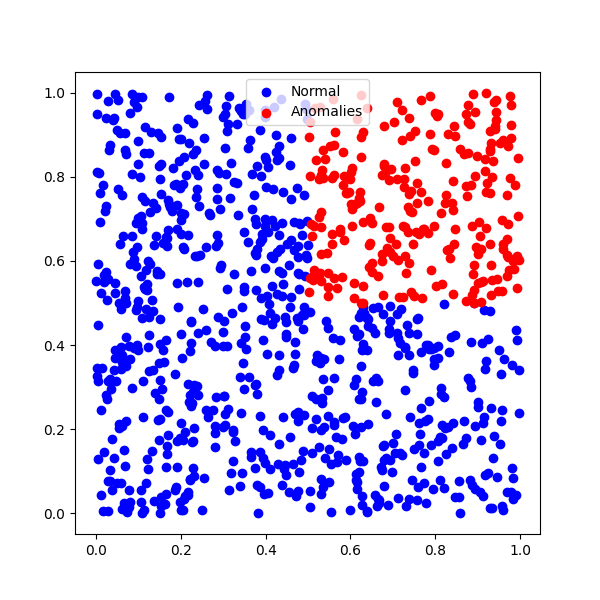
\includegraphics[width=0.45\textwidth]{images/norm_ano_ex.png}
  \caption{Plot of two features $f_1$ and $f_2$. Blue points are normal $N_i$ and red points are anomalies $A_i$.}
  \label{fig:exstream2dplot}
\end{figure}
This example was specifically chosen but we see that in practice the submodular property is also broken. This property depends on the function being used to compute the entropy. Meaning that with a well chosen function it is possible that the submodular property holds. However, this function would loose a lot of information and would not choose the optimal selection of features.\\
In conclusion we have proven that the submodular property does not hold for our data. This implies that we do not have an efficient way of finding the best set of features even with a multi dimensional entropy measure.\\
\subsection{Methods for generalizing Entropy}
Generalizing the computation of entropy to higher dimensions isn't trivial. The measure of entropy is done after creating clusters. In one dimension this is simply done by taking segments containing the same type of points. The number of points in each segment is then used to compute the entropy.\\
In higher dimensions we wish to keep a similar method. In order to do so we will thus only need to determine the optimal clustering method to be used.\\
There are certain properties that our clustering method must have in order to make sure it works properly.
\begin{itemize}
  \item It must obtain a similar result to Exstream when applied to a single feature.
  \item It must classify discontinue points into different clusters. Meaning that if there exists an anomalous point in between two normal points, these two normal points should be in different clusters.
  \item The method must generalize to higher dimensions. The number of dimensions can be limited to $\approx10$ as explained above this would be too long and wouldn't be useful.
  \item The method must fit any distribution of the data and work on few points.
  \item It must be possible to find intervals for the anomalies being clustered.
  \item The computational complexity of the method must not be "too" high. This is a vague requirement but it is important to keep in mind that the method will be used in a real time setting and will need to be evaluated on many sets of features. An exponential growth in complexity in the number of points would for example make the method unusable.
\end{itemize}
We will now present a few methods that could be used to cluster the data.
\subsubsection{Boxes}
\begin{figure}[H]
  \centering
  \begin{subfigure}{0.27\textwidth}
      \centering
      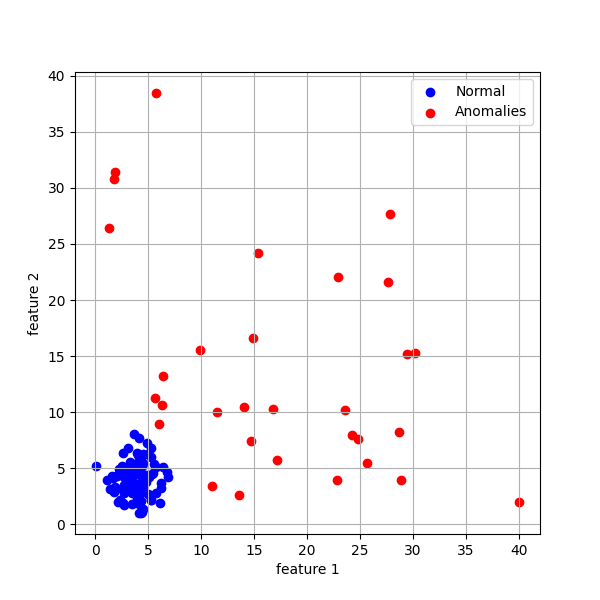
\includegraphics[width=\linewidth]{images/cubepoints.png}
      \caption{Points in the space}
  \end{subfigure}
  \hfill
  \begin{subfigure}{0.35\textwidth}
      \centering
      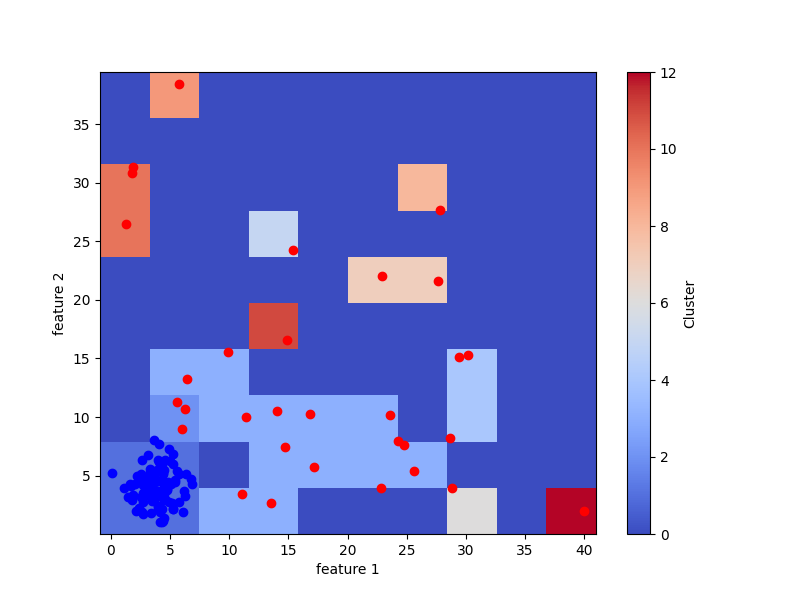
\includegraphics[width=\linewidth]{images/bad clustercube2.png}
      \caption{Clustering using 10x10 bins}
  \end{subfigure}
  \hfill
  \begin{subfigure}{0.35\textwidth}
      \centering
      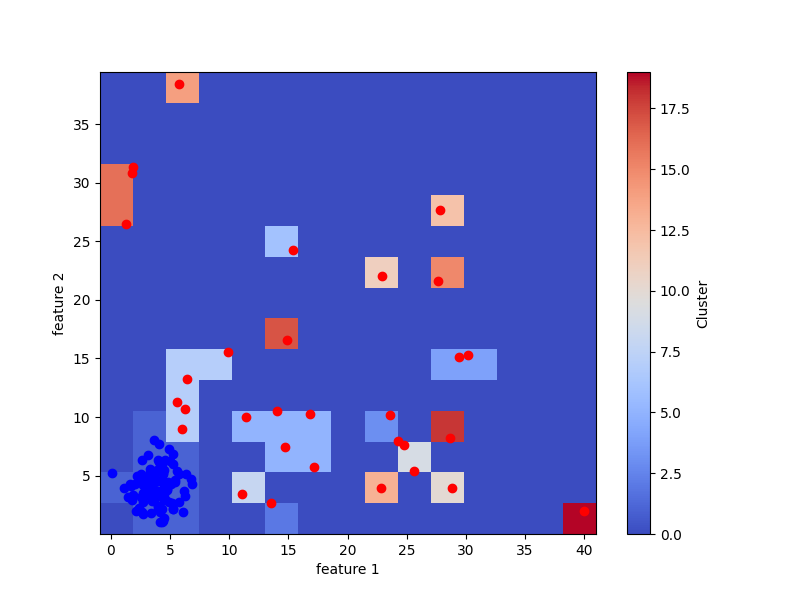
\includegraphics[width=\linewidth]{images/bad clustercube1.png}
      \caption{Clustering using 15x15 bins}
  \end{subfigure}
  \caption{Plot of points being clustered by using the Box method. Same coloured squares are in the same cluster.}
\end{figure}
The first method is inspired by the bin method for Exstream \cite{MijaExstream} presented above. The idea of dividing the feature space into bins to discretize the data can be easily generalized to higher dimensions. We would use n dimensional cubes to divide the space. We would then check the points in each cube and notate them as either normal, anomalous or mixed. Having done that, we would then merge adjacent cubes of the same type unless they are mixed in which case it isn't usefull to merge them. This would give us the clusters we need to compute the entropy.\\
This method has the merit of being simple and computationally efficient running in $O(n)$ time with n being the number of points considered. However, this method does not generalize well to higher dimensions and to different distributions of the data.\\
For example in the case with outlying points, as it is expected with anomalous data, the method would not be able to correctly merge the cubes. This would lead to a high number of clusters and a high entropy. The clusters are also highly dependent on the number of bins. The ideal number is impossible to know in advance and can be different per dimension and per trace.\\
Overall this method can work on simple data but isn't resilient enough for our use.\\


\subsubsection{Nearest neighbours}
\begin{figure}[H]
  \centering
  \begin{subfigure}{0.35\textwidth}
      \centering
      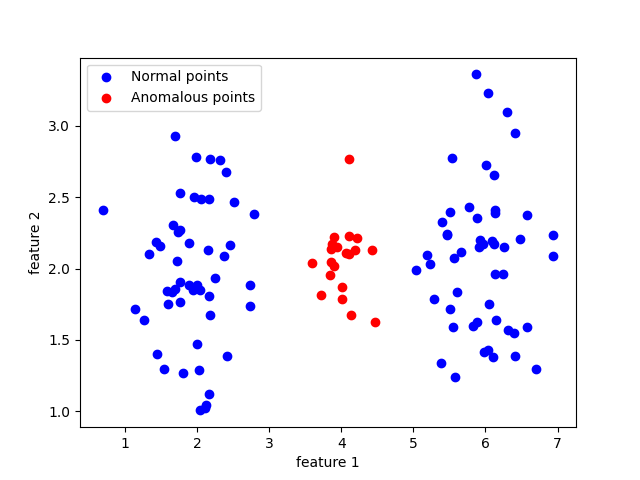
\includegraphics[width=\linewidth]{images/clustnn.png}
      \caption{Points in the space}
  \end{subfigure}
  \begin{subfigure}{0.35\textwidth}
      \centering
      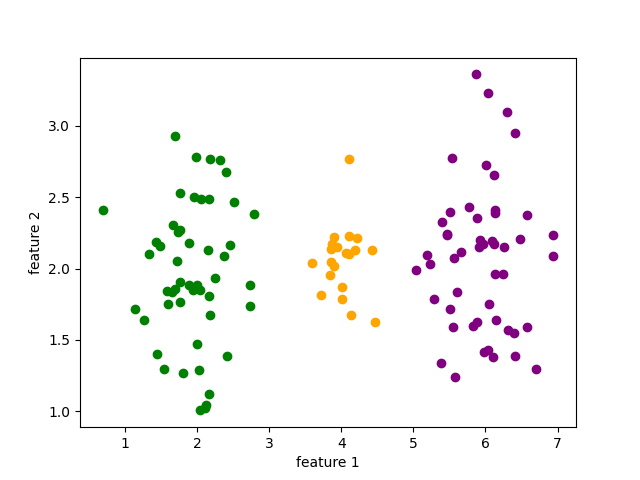
\includegraphics[width=\linewidth]{images/actual_nn.png}
      \caption{Clustering of the points.}
  \end{subfigure}
  \caption{Plot of points being clustered by using the nearest neighbours method. Same coloured points are in the same cluster.}
  \label{fig:nn_sep}
\end{figure}
\begin{figure}[H]
  \centering
  \begin{subfigure}{0.33\textwidth}
      \centering
      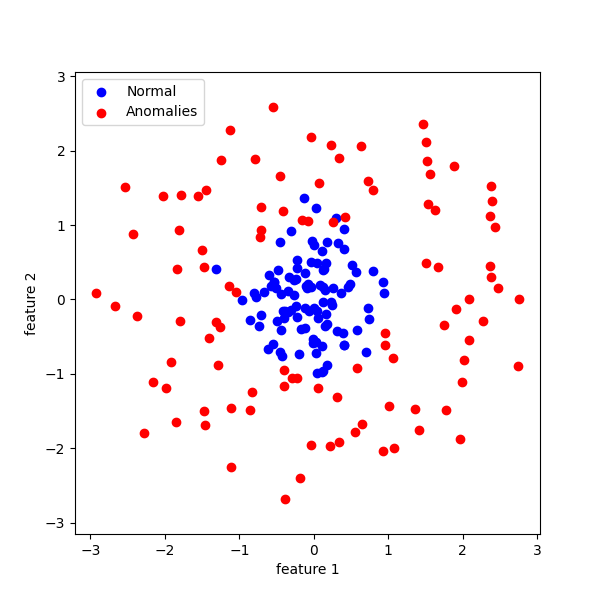
\includegraphics[width=\linewidth]{images/or_class_nn_circle.png}
      \caption{Points in the space}
  \end{subfigure}
  \begin{subfigure}{0.35\textwidth}
      \centering
      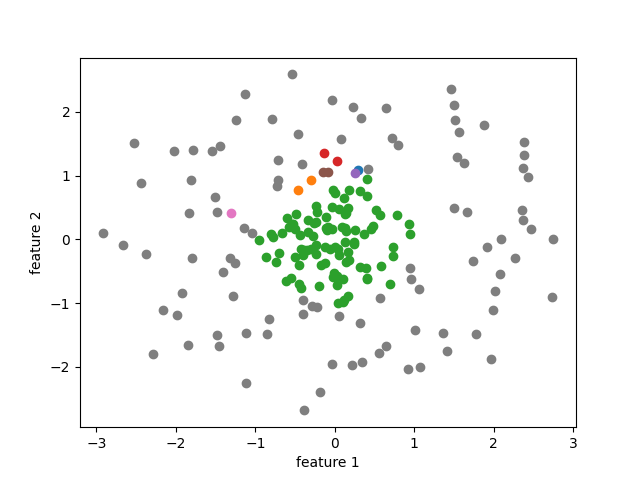
\includegraphics[width=\linewidth]{images/actual_nn_circle.png}
      \caption{Clustering of the points.}
  \end{subfigure}
  \caption{Plot of points being clustered by using the nearest neighbours method. Same coloured points are in the same cluster.}
  \label{fig:nn_circle}
\end{figure}
This method can be applied to single points or as an improvement to the post processing of the box method. It relies on the nearest neighbours of each points and is inspired directly by the property stating that we must "classify discontinue points into different clusters".\\
The method is as follows. For each points, we will iteratively get it's next nearest neighbour until reaching a point of the other class. We will cluster these points together. On top of that we merge clusters if a point is already part of a cluster. This method makes it so if two clusters are discontinue, meaning a point of the other class is placed in between them, they won't be merged together. See \autoref{fig:nn_sep}.\\ 
In practice we will use a KDtree for storing points and efficiently get the nearest neighbours. We will also restrict the maximum number of neighbours being considered in order to improve the efficiency.\\
Let $n$ be the number of points and $k$  a hyper parameter being the maximum number of neighbours. The KDtree is created in $O(n \log(n))$, the nearest neighbours are then computed in $O(k n\log(n))$ and the clustering is done in $O(n)$. Overall the method runs in $O(n \log(n))$ time. The method is therefore efficient and can be used in real time.\\
The method obtains the same results as Exstream on a single feature. It also generalizes well to higher dimensions and different distributions of the data as only the segmentation thereof is considered when clustering. The method is relatively stable with respect to the hyper parameter $k$, the only case where it would matter is for a group of isolated points of size greater than k. Those could be clustered together but not with the rest of the group.\\
The big issue with this method is the lack of intervals being determined. We only get points in clusters. These clusters aren't based on intervals. For example \autoref{fig:nn_circle} shows a case where the gray class doesn't translate to a clear interval. This is an issue as intervals strengthen the explanation and give much more information about the anomaly.
\subsubsection{Decision Trees}
\begin{figure}[H]
  \centering
  \begin{subfigure}{0.35\textwidth}
      \centering
      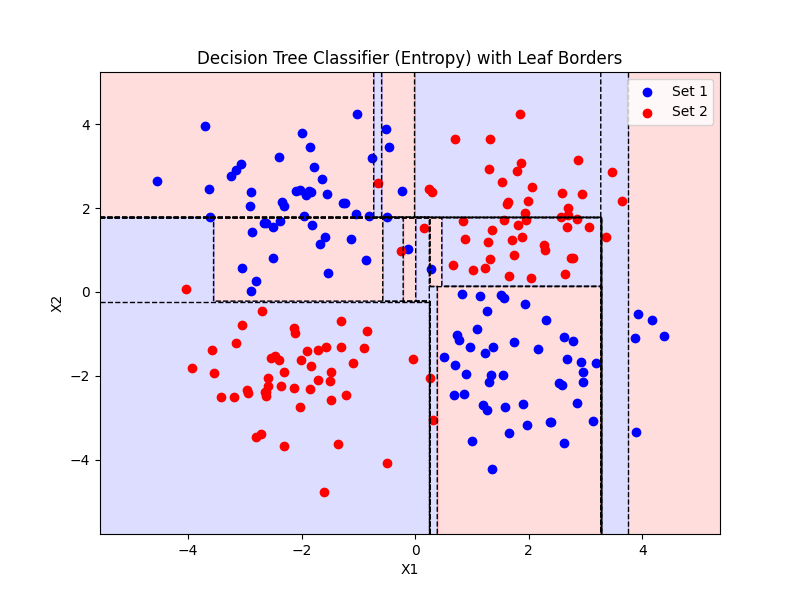
\includegraphics[width=\linewidth]{images/tree_border.png}
      \caption{Clustering of points.}
  \end{subfigure}
  \begin{subfigure}{0.35\textwidth}
      \centering
      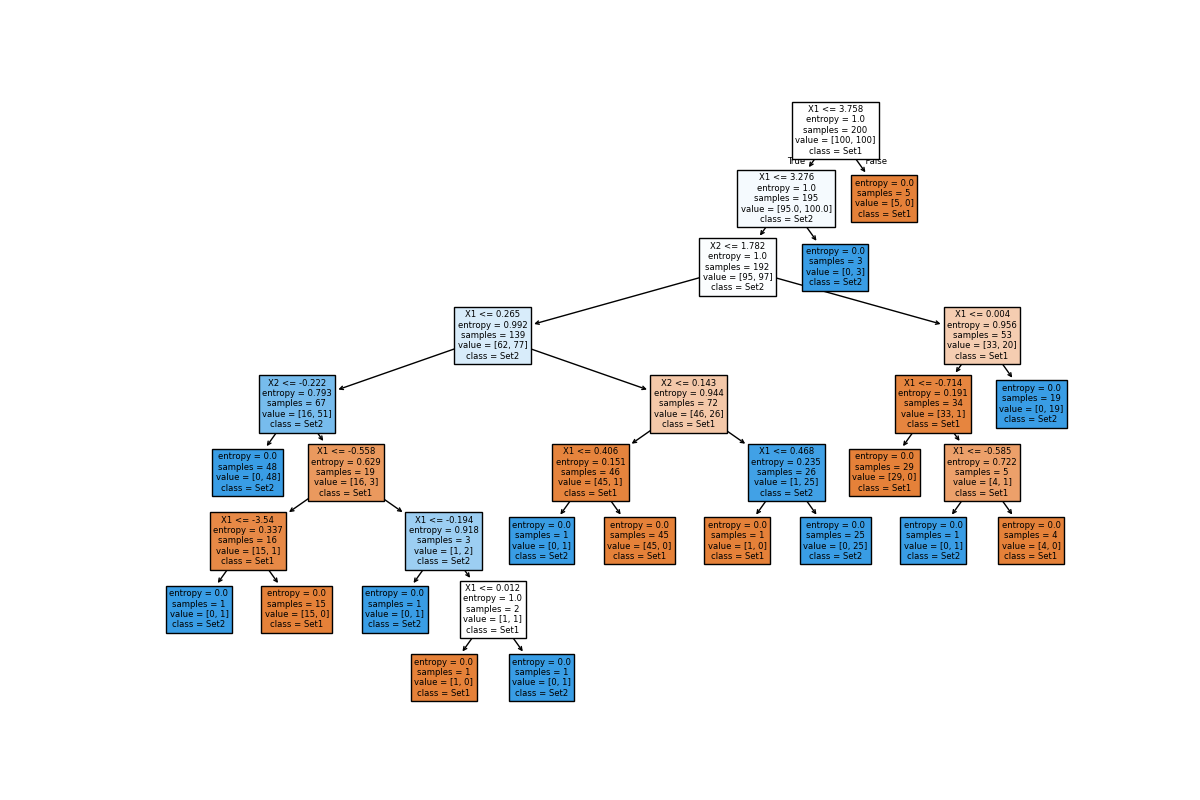
\includegraphics[width=\linewidth]{images/decision_tree.png}
      \caption{Corresponding decision tree.}
  \end{subfigure}
  \caption{Clustering of points and corresponding decision tree. Red points are anomalous and blue are normal. The lines mark the separation between clusters.}
  \label{fig:decision_tree}
\end{figure}
The final method we will present is the use of decision trees to cluster points. The idea is to train a decision tree on the two sets of points we have. We then use the leaves of the tree as clusters. Intuitively, a decision tree splits the space into hypercubes. Each node splits the space in two along a certain feature. The leaves are a conjunction of these splits, in essence creating a hypercubes subset of the space being considered. \\
In theory, the decision tree can split the space until each leaf is pure, i.e it contains only points of the same class. This would give us the optimal clustering. However, in practice we will allow the tree to split until having at minimum $k$ points in each leaf. Mixed clusters are then handled similarly as in Exstream and given the maximum segmentation score. This is done for efficiency purposes. It is also important to note that this limitation does not impact significantly the results. Reaching this limit would mean that the points are very segmented and that the entropy would be high in any case.\\
Now let us go over the properties of this method: 
\begin{itemize}
  \item The results are the same as Exstream when run on a single feature if we do not take into consideration the $k$ point approximation when the points are too segmented.
  \item Points are classified using Hypercubes. Therefore two points being classified in the same cluster means there are no points of the other class in between them. At the same time, two normal clusters with anomalous points in between cannot be classified together as the hypercube containing them would be impure.
  \item As most models, decision trees suffere from the curse of dimensionality. However in our case the number of dimensions considered is low and the method would work fine.
  \item A decision tree can fit any distribution. In our case we do not care about overfitting as we will not make predictions with it and only use it to cluster points.
  \item As stated previously, Decision trees create hypercubes. This in effect gives us intervals.
  \item We fit a decision tree on the data. This is done in $O(m n \log(n))$ with m being the number of dimensions and n being the number of points. In practice, the algorithm runs slightly faster than the nearest neighbor one. Overall the time complexity isn't too high.
\end{itemize}
This clustering method checks all of the properties we needed making it a good candidate for our use. The construction of the decision tree case be done using Gini impurity or entropy. We will use entropy as this creates a link between the creation of the tree and the measure we are trying to compute. At each node of the tree, the best split is created by minimizing the entropy of the two leaves created. This suits us as we are trying to minimize the entropy of the clusters.\\
The use of hypercubes for clustering provides intervals for our explanation. However, this implies that some points that are adjacent will fall in multiple clusters. For example in \autoref{fig:exstream2dplot}, the normal points will be split into two clusters. This can either be seen as a limitation or as a strength of this method. This penalizes the use of multiple dimensions when explaining the anomaly. Higher dimensions implie more cuts. This will prevent the incorporation of irrelevant features as these would either decrease the entropy or not change it. A byproduct of this is that getting a score of 1 for n features implies that there is a feature alone in that set that gets a score of 1. i.e let $g_i$ be the entropy function on segment $i$. $f_j$ is a feature for $j\in[1, n]$.:
\begin{align*}
  g_i([f_1, f_2, ..., f_n]) = 1 \Rightarrow \exists j \in [1, n], g_i([f_j]) = 1
\end{align*}
This is due to the fact that getting an entropy score of 1 implies that the points are perfectly segmented, thus finding 2 clusters. Using decision trees this implies a single cut along one dimension. Therefore the feature on which this cut was done is enough on its own to perfectly segment the points.\\
It is also possible to overcome this limitation by merging neighbouring leaves into one cluster. The intervals would still be given separately but the clusters would be considered as one, lowering the overall entropy. This would be done by checking the neighbouring leaves and merging them if they contain points of the same class. This would be done iteratively until no more merges are possible.\\
Decision trees also do not have any garantees of finding the best clusters. The method is greedy and will only split the space along the best feature at each node. This can lead to suboptimal clustering as for example in \autoref{fig:decision_tree}, the normal points on the right are split off early and are separated from the rest whereas they could have been clustered together. However, in practice the method works well and the results are satisfactory.\\
\subsection{Incorporation into Exstream}
We will now see how to incorporate any method mentioned above for computing entropy into Exstream. The intuitive way would be finding the set of features that obtains the best score through our method. However, as shown previously, finding such a set of features isn't a submodular optimization problem. We therefore do not have an efficient way of finding the best set of features. There might be other ways of finding the best set of features using properties of the different functions. However, in this paper we will not explore these. And will limit ourselves to brute forcing the problem in two dimensions.\\
Another cause to motivate this decision of keeping the number of features considered to two is the complexity of our dataset and of the anomaly types. There are many traces where a single feature alone has perfect separation between the normal and anomalous points getting an entropy score of 1. Moreover, some traces contain multiple such features that are not heavilly correlated. In these cases it is useless to search for a combination of feautres as a single feature alone has a perfect score. It is also above the scope of this work to improve the selection of features to be returned in the above case. We will therefore rely on the same method as Exstream and when a feature gets a score above a certain threshold, we will not search in two dimensions and return all features with a score above that threshold subject that they are not correlated and that they are not false positives.\\
The returned format for the anomalous intervals will be the same as in the original exstream with $I^i_j$ intervals: 
\begin{align*}
  ((f_1 \in I^1_1 \lor f_1 \in I^1_2 ...) \land (f_2 \in I^2_1 \lor f_2 \in I^2_2 ...)) ...
\end{align*}
The case where no single feature is enough to perfectly segment the normal and anomalous points, we will brute force the problem in two dimensions. After removing false positive feature, we will compute the entropy for all pairs of features and return the pair that has the best score. Considering there are initially 237 features in the dataset, in the worst case (when there aren't any false positive features), we will be computing the entropy for ${237\choose2} = \frac{237 \times 236}{2} = 27966$ pairs of features. This is a lot of computation especially considering the complexity for each pair is $O(n \log(n))$. \\
When using the decision tree method, we will obtain hypercubes as intervals. These hypercubes can be defined as the conjunction of intervals in each feature. Therefore the return format will be the following: 
\begin{align*}
  (f_1 \in I^1_1 \land f_2 \in I^2_1) \lor (f_1 \in I^1_2 \land f_2 \in I^2_2) ...
\end{align*}
This inversion between $\land$ and $\lor$ provides much more information about specific intervals where points are anomalous. It is also possible to return multiple pairs as explanation. These would be linked using $\land$ clauses.\\
The new output format will be the following:
\begin{verbatim}
{
  "Trace":{
    "Anomaly number and type":{
      "feature_to_importance":{
          "feature_1, feature_2": score
      },
      "feature_to_intervals":{
          "feature_1, feature_2":[
              [
                  [
                      feature_1 start,
                      feature_2 start
                  ],
                  [
                      feature_1 end,
                      feature_2 end
                  ],
                  include starts,
                  include ends
              ],
              ...
          ]
      }
    },
    ...
  }
  ...
}
\end{verbatim}
\subsection{Results}
\begin{table}[h]
  \centering
  \begin{tabular}{|c|c|c|c|c|c|c|}
      \hline
      Methods & Time & Length & Instability & Discordance & ED1 F1 Score & ED2 F1 Score\\ 
      \hline
      Exstream  & 1.5  & 1.6  & 2.26  & 7.71 & 0.88 & 0.87  \\ 
      Exstream 80\% & 1.1 & 3.4 & 2.0 & 5.5 & 0.88 & 0.90 \\
      Exstream 90\%  & 1.2  & 2.4  & 1.88  & 6.04 & 0.88 & 0.92\\ 
      Exstream 95\%  & 1.35  & 2.1  & 2.08  & 6.59 & 0.87 & 0.93\\ 
      Exstream Bins  & 140.7  & 4.3  & 1.5  & 6.16 & 0.79 & 0.72 \\ 
      Exstream Tree 80\%  & 15.6 & 2.9  & 1.63 & 5.76 & 0.997 & 0.94 \\ 
      Exstream Tree 90\%  & 29.3  & 1.9  & 1.91 & 6.91 & 0.997 & 0.96 \\ 
      Exstream Tree 95\%  & 55.2  & 1.5  & 2.22 & 8.43 & 0.997 & 0.97 \\ 
      \hline
  \end{tabular}
  \caption{Results of evaluating the new method}
  \label{tab:results_tree}
\end{table}
This new method is evaluated with the same metrics as the original Exstream and on the same traces. We shall also evaluate the method while removing the beginning and end 10\%, 5\% and 2.5\% of each normal and anomalous instance. The results are presented in \autoref{tab:results_tree}.\\
An improvement in the length of the explanation along with a worsened discordance can be observed. This is due to the way the output is handled. A pair of features $(f_1, f_2)$ is considered a single conjunction. Therefore, in disjunctive normal form it is counted as a single feature. Therefore whenever any single feature doesn't get a high enough score, the length of the explanation will be one. One the other hand, each pair is considered a unique new feature. This is why the discordance is higher.\\
The F1 score in ED1 and ED2 settings are both improved significantly using this new method. This is due to the fact that the method is able to capture the interaction between features and express intervals in a more precise way. This result is very satisfactory as it shows that 
\begin{figure}[H]
  \centering
  \begin{subfigure}{0.30\textwidth}
      \centering
      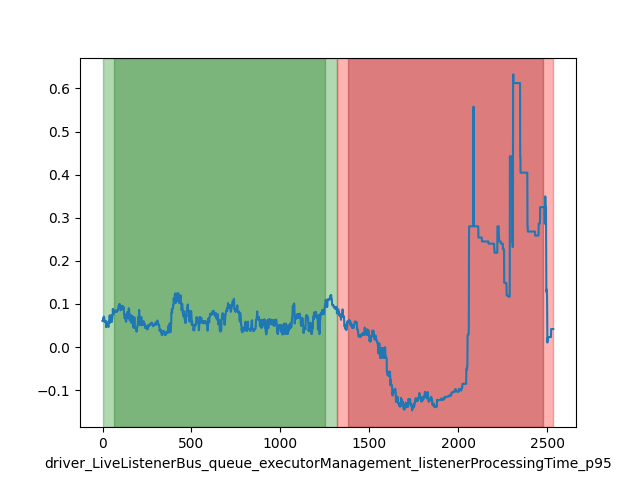
\includegraphics[width=\linewidth]{images/plotduo1111.png}
      \caption{Feature 1}
  \end{subfigure}
  \begin{subfigure}{0.30\textwidth}
      \centering
      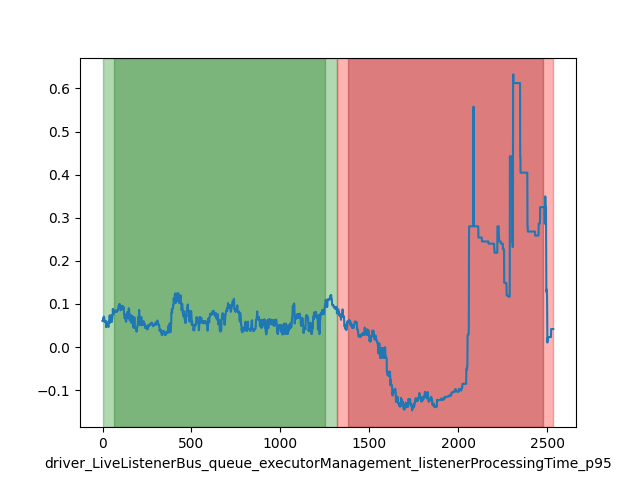
\includegraphics[width=\linewidth]{images/plotduo1111.png}
      \caption{Feature 2}
  \end{subfigure}
  \begin{subfigure}{0.30\textwidth}
    \centering
    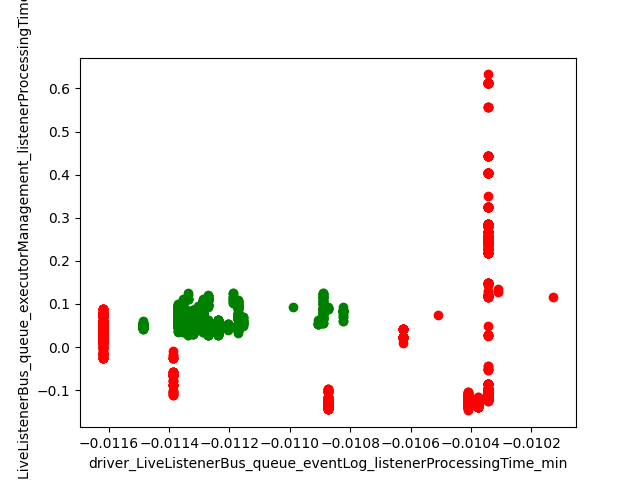
\includegraphics[width=\linewidth]{images/scatter duo.png}
    \caption{Scatterplot of normal and anomalous points. Red are anomalous and green normal.}
\end{subfigure}
  \caption{Example of Explanation using two features. Trace 8\_4\_1000000\_10\_2\_15\_77 3T4}
  \label{fig:decision_tree}
\end{figure}
\section{Conclusion}
We have first presented a method to improve the sampling of points. This method is restricted by the existence of domains. We therefore used reconstructed points. This methods doesn't provide the expected results. We then presented a method to generalize the entropy measure to higher dimensions. We showed that the submodular property doesn't hold for our data. We then presented three methods to cluster points in higher dimensions. The decision tree method was chosen as it fits all the requirements we had. We then showed how to incorporate this method into Exstream. The results show a significant improvement in the F1 score. The length of the explanation is also improved. The discordance is worsened but this is due to the way the output is handled. The method is also evaluated on different traces and different percentages of points removed. The results are consistent and show a significant improvement.\\
Overall, even though our first endeavour in improving the sample of points wasn't successful, the second method of generalizing Exstream in higher dimensions was. The results are very satisfactory and show that the method is able to capture the interaction between features and provide a more precise explanation.\\
\section{Further works}
\begin{figure}[H]
  \centering
  \begin{subfigure}{0.30\textwidth}
      \centering
      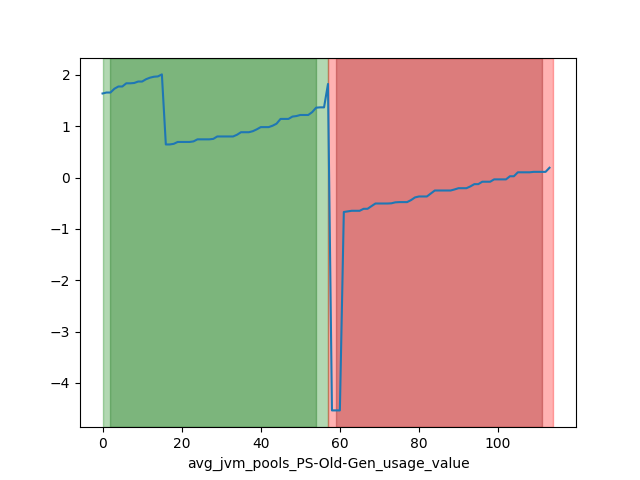
\includegraphics[width=\linewidth]{images/ex0.png}
      \caption{Feature 1}
  \end{subfigure}
  \begin{subfigure}{0.30\textwidth}
      \centering
      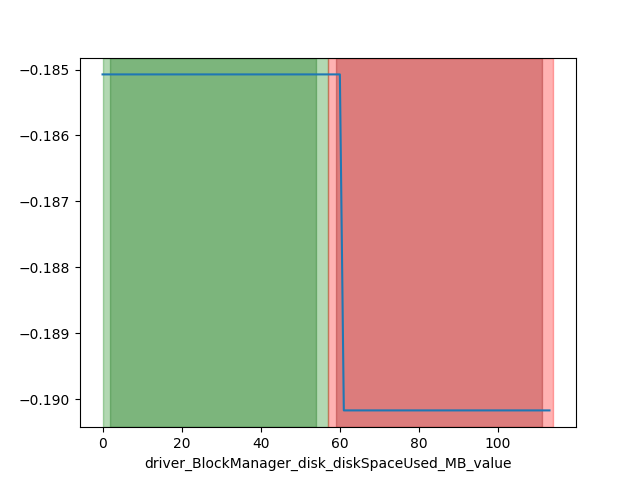
\includegraphics[width=\linewidth]{images/ex1.png}
      \caption{Feature 2}
  \end{subfigure}
  \begin{subfigure}{0.30\textwidth}
    \centering
    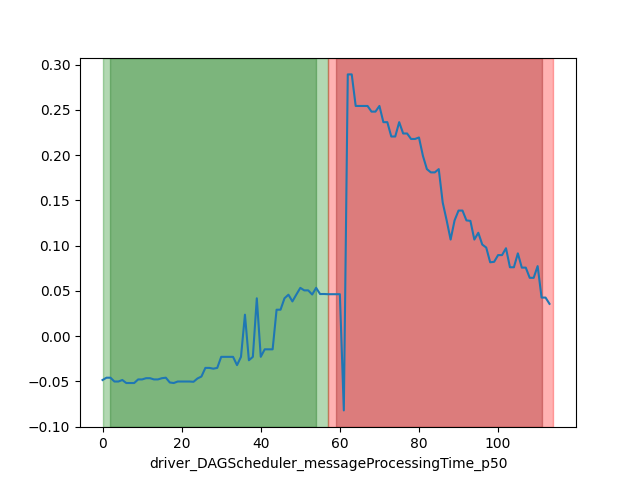
\includegraphics[width=\linewidth]{images/ex3.png}
    \caption{Feature 3}
\end{subfigure}
\begin{subfigure}{0.30\textwidth}
  \centering
  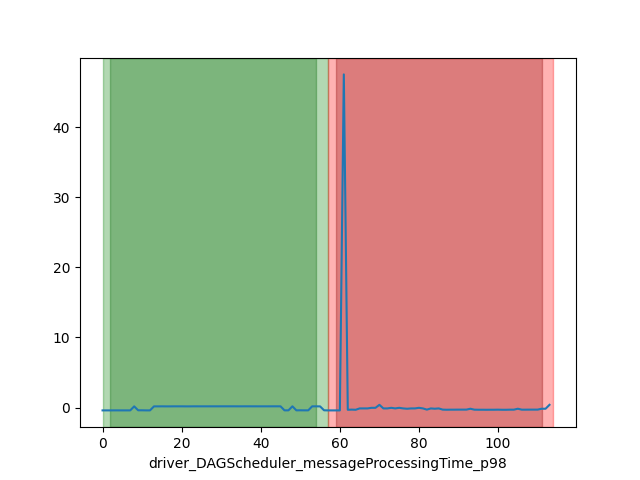
\includegraphics[width=\linewidth]{images/ex4.png}
  \caption{Feature 4}
\end{subfigure}
\begin{subfigure}{0.30\textwidth}
  \centering
  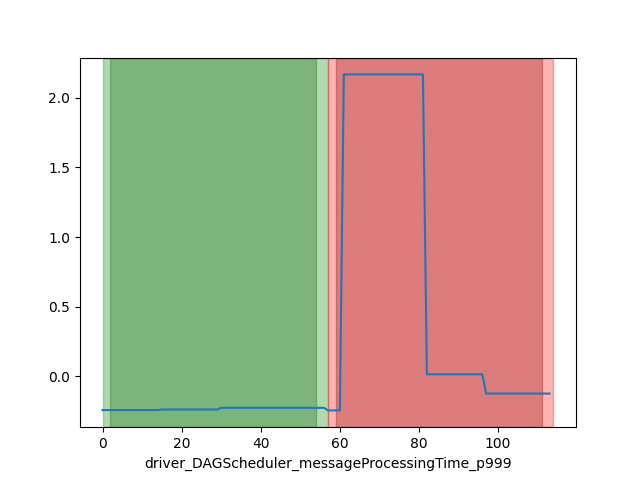
\includegraphics[width=\linewidth]{images/ex5.png}
  \caption{Feature 5}
\end{subfigure}
\begin{subfigure}{0.30\textwidth}
  \centering
  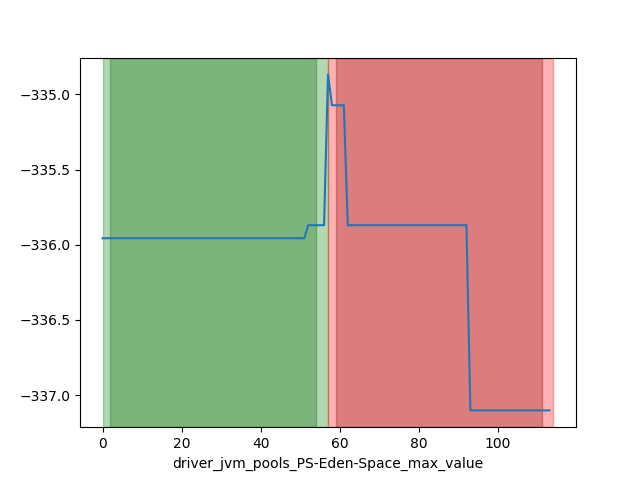
\includegraphics[width=\linewidth]{images/ex6.png}
  \caption{Feature 6}
\end{subfigure}
  \caption{Example of Explanation using six features. Trace 5\_5\_1500000\_5\_3\_15\_92 1T5}
  \label{fig:sixexpl}
\end{figure}
The length of the explanations are longer than in the original Exstream. There are still explanations with 5 or 6 features. For example \autoref{fig:sixexpl}, we have 6 features with each a score of 1. These features were not detected as being correlated. This number of features is too much in an explanation and some features might be correlated with each other while not being detected in the restricted sample which we have. Moreover, if features $f_1$ and $f_2$ are correlated, if $f_1$ is returned as explanation in one anomaly and $f_2$ in another, the discordance will increase. We could therefore find a way to always return the same features when they are correlated. This motivates the grouping of \textit{globally} correlated features whith a set rule on which to return as explanation.\\\\
The method we introduced to sample using the latent space isn't satisfactory. The features correlated with time are thus still not detected and removed. This is something to work on and improve in the future.\\\\
Our method using trees is currently limited to two dimensions. This is enough on our dataset that is simple. However, in a more complex dataset, the method would need to be generalized to more dimensions. The limitation is due to the way we search for the best set of features in a brute force manner. This is innefiscient and limits the search in higher dimensions. We could find a way to efficiently search for the best set of features in higher dimensions. This would enable the method to be used on more complex datasets.\\\\


\newpage
\bibliographystyle{plain}
\bibliography{main}

\newpage
\appendix

\section{Appendix}
\label{sec:appendix}


\begin{figure}[h]
    \centering
    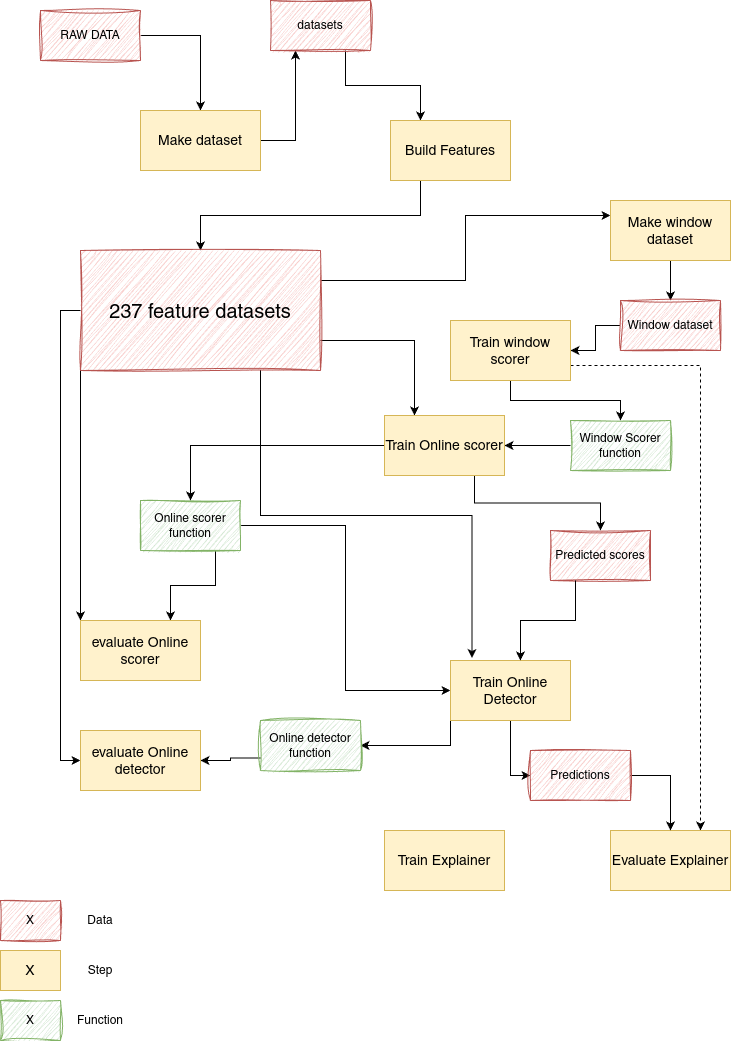
\includegraphics[width=0.7\textwidth]{images/pipeline.drawio.png} % Replace with your image file name
    \caption{Pipeline of Exathlon}
    \label{fig:pipeline}
\end{figure}
\begin{figure}[h]
  \centering
  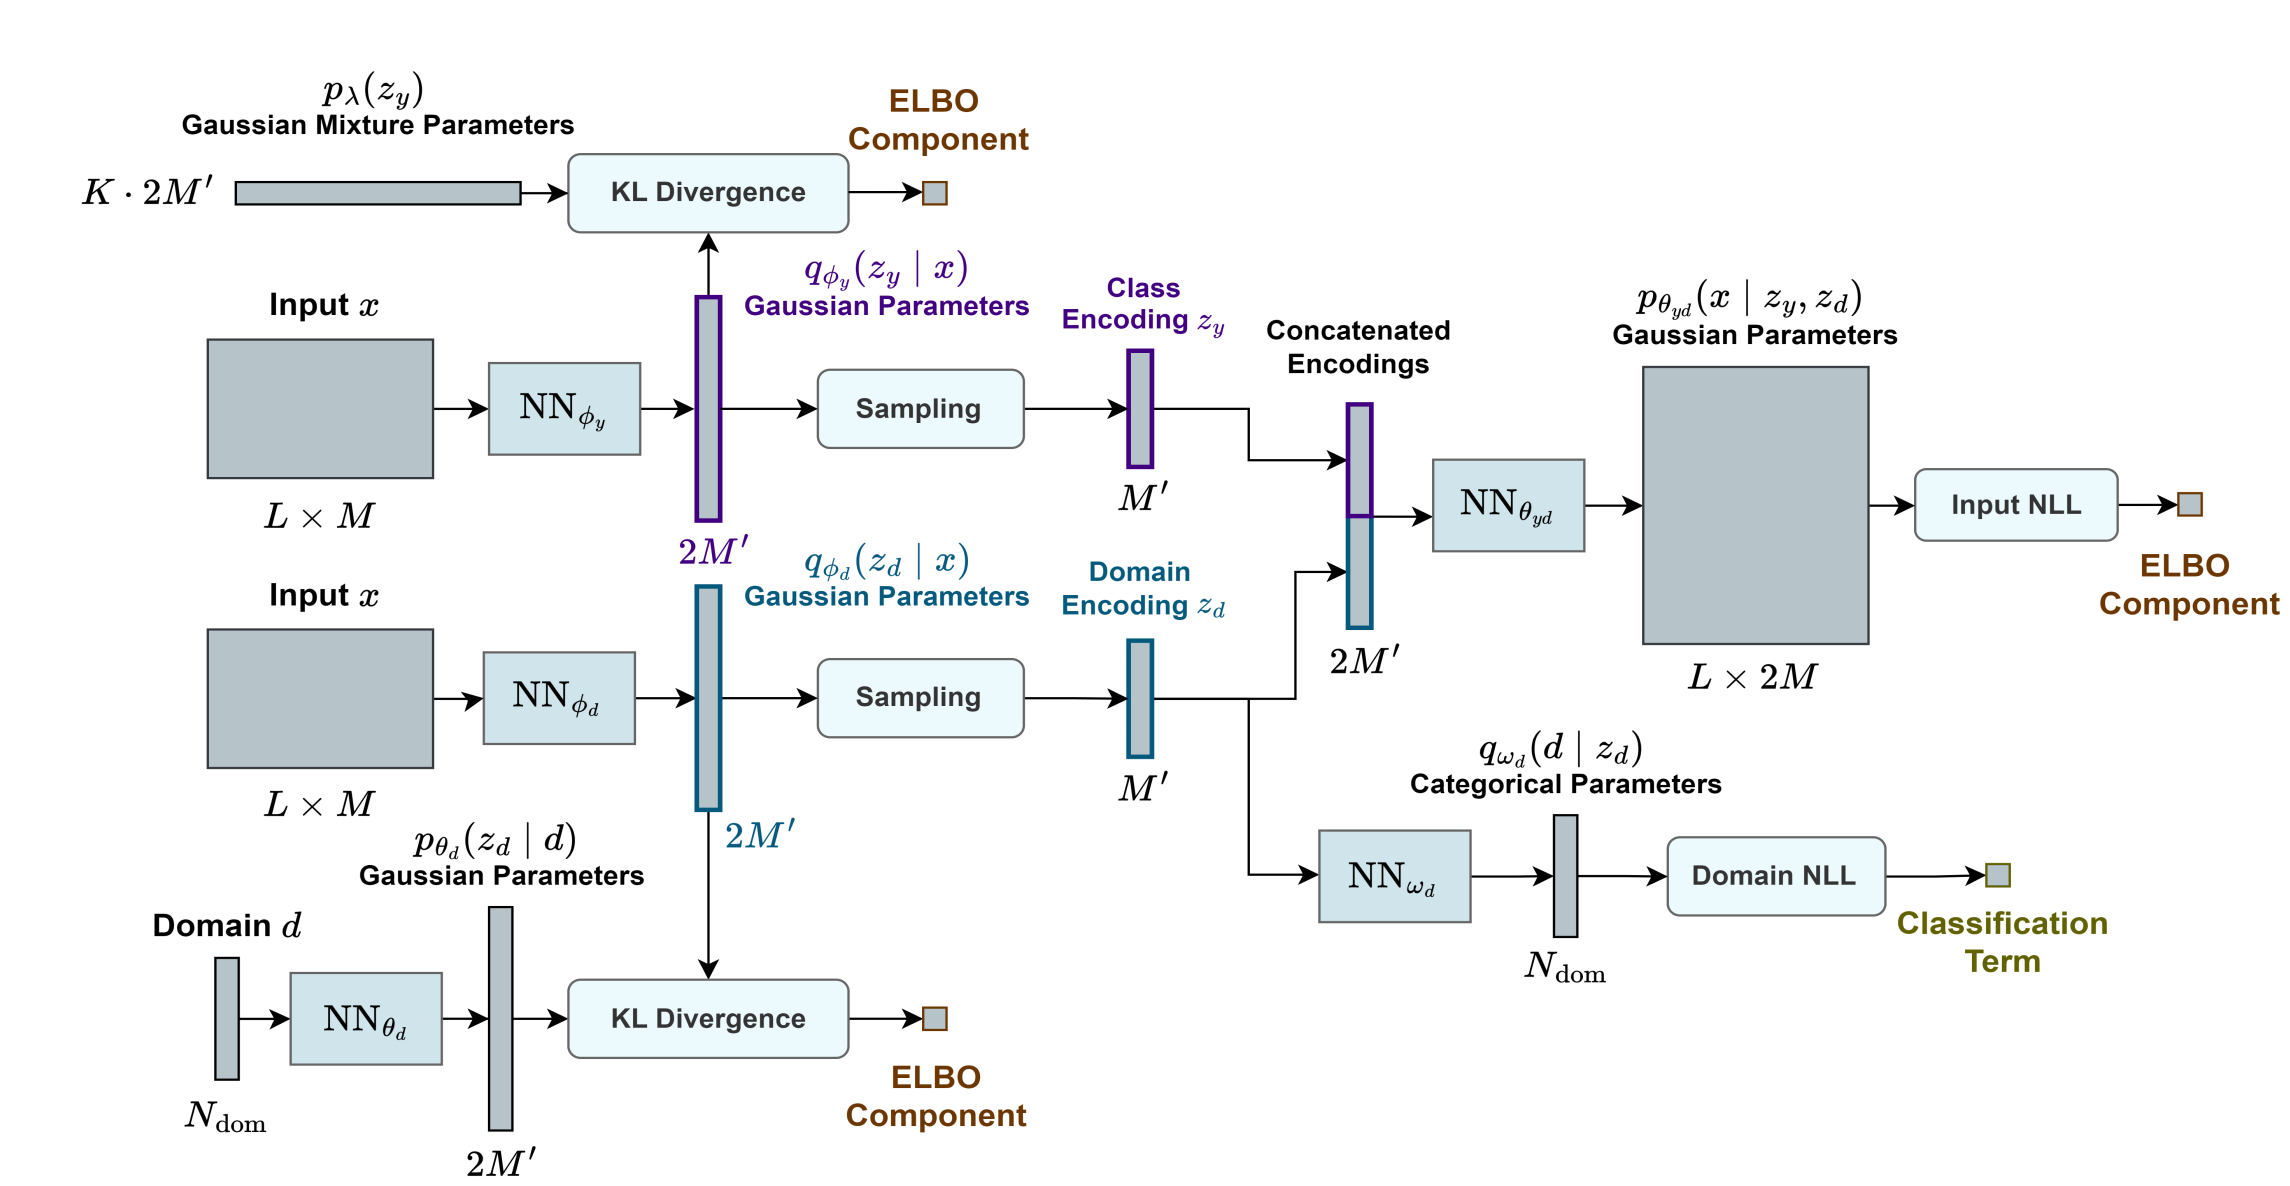
\includegraphics[width=1\textwidth]{images/divad model.png} % Replace with your image file name
  \caption{Divad model architecture}
  \label{fig:divad_arch}
\end{figure}
\end{document}
